\section{Proofs in \protect\NoCaseChange{\cref{sec:pid}}}\label{app:proofs_pid}

\subsection{Proof of Sharpness}

\begin{proof}[Proof of \cref{prop:sharpness}]
    \noindent\textbf{Direct direction.}
    Let $\tilde{\pi}$ be a probability measure on $\mathcal{Y}^2 \times [0,1] \times \mathcal{X}$ whose $(Y(w), U, X)$-marginals satisfy $(\tilde{\pi}_0,\tilde{\pi}_1) \in \Gamma(\mathbb{P}_{\text{obs}})$. By the constraints in~(\ref{eq:ot_formulation}), each $\tilde{\pi}_w$ is a probability measure on $\mathcal{Y} \times [0,1] \times \mathcal{X}$ satisfying:
    \begin{enumerate}
        \item[(C1)] $\displaystyle \int_0^{p(z,x)} \tilde{\pi}_1(\mathrm{d}y \mid u, x) \, \mathrm{d}u = H_{1,x}(p(z,x),\mathrm{d}y)$, for $\mathbb{P}_{\text{obs}}$-a.e.\ $(z,x)$;
        \item[(C2)] $\displaystyle \int_{p(z,x)}^{1} \tilde{\pi}_0(\mathrm{d}y \mid u, x) \, \mathrm{d}u = H_{0,x}(p(z,x),\mathrm{d}y)$, for $\mathbb{P}_{\text{obs}}$-a.e.\ $(z,x)$;
        \item[(C3)] $\tilde{\pi}_w(\mathrm{d}u, \mathrm{d}x) = \mathrm{d}u \, \mathbb{P}_{\text{obs}}(\mathrm{d}x)$ for $w \in \{0,1\}$.
    \end{enumerate}
    Since $\mathcal{Y}^2 \subseteq \mathbb{R}^2$ is a Polish space and the $(U, X)$-marginal of $\tilde{\pi}$ is $\mathrm{d}u \, \mathbb{P}_{\text{obs}}(\mathrm{d}x)$ by (C3) applied to either marginal, $\tilde{\pi}$ admits a regular conditional kernel $\tilde{\pi}(\mathrm{d}y_0, \mathrm{d}y_1 \mid u, x)$ for $(\mathrm{d}u \otimes \mathbb{P}_{\text{obs}}(\mathrm{d}x))$-a.e.\ $(u, x)$, whose $Y(0)$- and $Y(1)$-marginals recover $\tilde{\pi}_0(\mathrm{d}y_0 \mid u, x)$ and $\tilde{\pi}_1(\mathrm{d}y_1 \mid u, x)$ respectively.

    \medskip
    \noindent\textbf{Construction.}
    We construct the joint distribution $\mathbb{P}$ of $(Y(0), Y(1), U, X, Z, W)$ on the product space $\mathcal{Y}^2 \times [0,1] \times \mathcal{X} \times \mathcal{Z} \times \{0,1\}$ via the following disintegration:
    \begin{equation}\label{eq:sharp_construct}
        \mathbb{P}(\mathrm{d}y_0, \mathrm{d}y_1, \mathrm{d}u, \mathrm{d}x, \mathrm{d}z, \{w\})
        = \tilde{\pi}(\mathrm{d}y_0, \mathrm{d}y_1 \mid u, x) \, \mathrm{d}u \, \mathbb{P}_{\text{obs}}(\mathrm{d}z \mid x) \, \mathbb{P}_{\text{obs}}(\mathrm{d}x) \, \delta_{\indicator(u \leqslant p(z,x))}(\{w\}),
    \end{equation}
    where $\delta_{\indicator(u \leqslant p(z,x))}(\{w\})$ is the Dirac mass placing all weight on $w = \indicator(u \leqslant p(z,x))$, enforcing the threshold-crossing selection rule deterministically. Crucially, $(Y(0), Y(1))$ are drawn jointly from $\tilde{\pi}(\cdot \mid u, x)$, so the coupling prescribed by $\tilde{\pi}$ is preserved conditional on $(U, X)$; the independent coupling $\tilde{\pi}_0(\mathrm{d}y_0 \mid u, x) \, \tilde{\pi}_1(\mathrm{d}y_1 \mid u, x)$ is one feasible choice among many. The measure in~(\ref{eq:sharp_construct}) is well-defined because the kernels are measurable and all component measures are probability measures.

    \medskip
    \noindent\textbf{Proof of (i): joint marginal distribution.}
    We show that the $(Y(0), Y(1), U, X)$-marginal of $\mathbb{P}$ equals $\tilde{\pi}$. Marginalizing~(\ref{eq:sharp_construct}) over $(Z, W)$:
    \begin{align*}
        \mathbb{P}(\mathrm{d}y_0, \mathrm{d}y_1, \mathrm{d}u, \mathrm{d}x)
        &= \tilde{\pi}(\mathrm{d}y_0, \mathrm{d}y_1 \mid u, x) \, \mathrm{d}u \, \mathbb{P}_{\text{obs}}(\mathrm{d}x) \underbrace{\sum_{w \in \{0, 1\}} \int_{\mathcal{Z}} \delta_{\indicator(u \leqslant p(z,x))}(\{w\}) \, \mathbb{P}_{\text{obs}}(\mathrm{d}z \mid x)}_{=\, 1} \\
        &= \tilde{\pi}(\mathrm{d}y_0, \mathrm{d}y_1 \mid u, x) \, \mathrm{d}u \, \mathbb{P}_{\text{obs}}(\mathrm{d}x).
    \end{align*}
    By (C3) the $(U, X)$-marginal of $\tilde{\pi}$ is $\mathrm{d}u \, \mathbb{P}_{\text{obs}}(\mathrm{d}x)$, so the right-hand side equals
    \begin{equation*}
        \tilde{\pi}(\mathrm{d}y_0, \mathrm{d}y_1, \mathrm{d}u, \mathrm{d}x),
    \end{equation*}
    establishing (i).

    \medskip
    \noindent\textbf{Proof of (ii): structural assumptions.}
    We establish each part of \cref{asp:structure}.
    \begin{itemize}
        \item \textbf{Consistency.} Consistency holds trivially by setting the observed outcome to be $Y = W Y(1) + (1-W) Y(0)$.
        \item \textbf{Conditional instrumental exogeneity.} By~(\ref{eq:sharp_construct}), conditional on $X = x$, the variables $(Y(0), Y(1), U)$ are drawn from $\tilde{\pi}(\mathrm{d}y_0, \mathrm{d}y_1 \mid u, x) \, \mathrm{d}u$ and $Z$ is drawn independently from $\mathbb{P}_{\text{obs}}(\mathrm{d}z \mid x)$. These appear as independent factors in~(\ref{eq:sharp_construct}), so $Z \indep (Y(0), Y(1), U) \mid X$ under $\mathbb{P}$.
        \item \textbf{Threshold crossing.} The selection equation $W = \indicator(U \leqslant p(Z,X))$ holds $\mathbb{P}$-a.s.\ by the Dirac mass in~(\ref{eq:sharp_construct}). Moreover, (C3) gives $U \mid X \sim \mathrm{Unif}(0,1)$. Conditional instrumental exogeneity then yields $\mathbb P(W=1\mid Z=z,X=x)=p(z,x)$ for $\mathbb P_{Z,X}$-almost every $(z,x)$.
        \item \textbf{Common instrument support.} The construction preserves the observed conditional law $\mathbb P_{\mathrm{obs}}(\mathrm dz\mid x)$. Because the proposition assumes that $\mathbb P_{\mathrm{obs}}$ is generated by a model satisfying \cref{asp:structure}, its common-support property is inherited by the constructed model.
    \end{itemize}

    \medskip
    \noindent\textbf{Proof of (iii): observational equivalence.}
    We must show that the distribution of the observables $(Y, Z, X, W)$ induced by $\mathbb{P}$ coincides with $\mathbb{P}_{\text{obs}}$. Since the marginal of $(Z, X)$ under $\mathbb{P}$ equals $\mathbb{P}_{\text{obs}}(Z, X)$ by construction, it suffices to show that the conditional laws of $(Y, W)$ given $(Z, X)$ agree.

    Fix $(z, x)$ and consider the event $W = 1$. Under $\mathbb{P}$, marginalizing~(\ref{eq:sharp_construct}) over $(Y(0), Y(1))$ reduces the joint kernel to its $Y(1)$-marginal $\tilde{\pi}_1(\cdot \mid u, x)$; using $W = 1 \Leftrightarrow U \leqslant p(z,x)$ and $Y = Y(1)$ when $W = 1$,
    \begin{align*}
        \mathbb{P}(Y \in A, \, W = 1 \mid Z = z, X = x)
        &= \int_0^{p(z,x)} \tilde{\pi}_1(A \mid u, x) \, \mathrm{d}u.
    \end{align*}
    By constraint (C1), this equals $H_{1,x}(p(z,x),A)$, which is the observed conditional subdistribution $\mathbb{P}_{\text{obs}}(Y \in A, \, W = 1 \mid Z = z, X = x)$ for $\mathbb P_{Z,X}$-almost every $(z,x)$. Similarly, for $W = 0$ we have $Y = Y(0)$ and $U > p(z, x)$, so marginalizing over $(Y(0), Y(1))$ leaves the $Y(0)$-marginal $\tilde{\pi}_0$ and
    \begin{align*}
        \mathbb{P}(Y \in A, \, W = 0 \mid Z = z, X = x)
        &= \int_{p(z,x)}^{1} \tilde{\pi}_0(A \mid u, x) \, \mathrm{d}u,
    \end{align*}
    which equals $H_{0,x}(p(z,x),A)$ by constraint (C2), and hence equals the corresponding observed conditional subdistribution almost surely. Thus the conditional laws of $(Y, W) \mid (Z, X)$ under $\mathbb{P}$ and $\mathbb{P}_{\text{obs}}$ agree for both values of $W$, which proves (iii).

    \medskip
    \noindent\textbf{Converse direction.}
    Suppose $(Y(0), Y(1), U, X, Z, W)$ is a joint distribution satisfying (ii)--(iii), and let $\tilde{\pi}$ denote its $(Y(0), Y(1), U, X)$-marginal. Fix $w \in \{0, 1\}$. The $(U, X)$-marginal of $\tilde{\pi}_w$ equals the $(U, X)$-marginal of $\tilde{\pi}$; by \cref{asp:structure} (threshold crossing), $U \mid X \sim \mathrm{Unif}(0, 1)$ and $X$ has marginal $\mathbb{P}_{\text{obs}}(\mathrm{d}x)$ under (iii), so $\tilde{\pi}_w(\mathrm{d}u, \mathrm{d}x) = \mathrm{d}u \, \mathbb{P}_{\text{obs}}(\mathrm{d}x)$, establishing (C3). For (C1), using consistency and the selection rule $W = \indicator(U \leqslant p(Z, X))$ together with conditional instrumental exogeneity,
    \begin{align*}
        \mathbb{P}_{\text{obs}}(Y \in A, \, W = 1 \mid Z = z, X = x)
        &= \mathbb{P}(Y(1) \in A, \, U \leqslant p(z, x) \mid Z = z, X = x) \\
        &= \int_0^{p(z, x)} \tilde{\pi}_1(A \mid u, x) \, \mathrm{d}u,
    \end{align*}
    where the second equality uses $Z \indep (Y(1), U) \mid X$ and $U \mid X \sim \mathrm{Unif}(0, 1)$. Property (iii) identifies the left-hand side with the observational conditional distribution. By the propensity-score sufficiency argument preceding~(\ref{eq:canonical_submeasures}), its canonical propensity-indexed version is $H_{1,x}(p(z,x),A)$, yielding (C1). The argument for (C2) is symmetric. Therefore $(\tilde{\pi}_0,\tilde{\pi}_1) \in \Gamma(\mathbb{P}_{\text{obs}})$, completing the converse.
\end{proof}

% The following discrete-case covariate proof is retained (commented out) for
% future reference. The unified proof of \cref{thm:covariate_continuous_lower_bound}
% below now covers this case as a special instance (every LIV interval degenerate).
\iffalse
\subsection{Proof of \cref{thm:covariate_discrete_lower_bound}}

\begin{proof}[Proof of \cref{thm:covariate_discrete_lower_bound}]
We prove the sharp lower bound; the upper bound follows by an identical argument with the comonotonic coupling replacing the countermonotonic one and swapping $y_{\min}$ and $y_{\max}$ in the trivial bound term.

\medskip
\noindent\textbf{Disintegration over $X$.}
Recall that the $W=1$ side minimization problem~(\ref{eq:ot_formulation_1}) reads
\begin{equation*}
    \min_{\pi_1 \in \Gamma_1(\mathbb{P}_{\text{obs}})} \mathbb{E}_{\pi_1}[Y(1)\,\omega(X,U)],
\end{equation*}
where $\Gamma_1(\mathbb{P}_{\text{obs}})$ denotes the set of probability measures $\pi_1$ on $\mathcal{Y} \times [0,1] \times \mathcal{X}$ satisfying
\begin{align}
    &\int_0^{p(z,x)} \pi_1(\mathrm{d}y \mid u, x)\,\mathrm{d}u = \mathbb{P}_{\text{obs}}(\mathrm{d}y, W\!=\!1 \mid p(Z,X)\!=\!p(z,x), X\!=\!x), \quad \text{for } \mathbb{P}_{\text{obs}}\text{-a.e.\ } (z,x), \label{eq:pf_constraint1} \\
    &\pi_1(\mathrm{d}u, \mathrm{d}x) = \mathrm{d}u\;\mathbb{P}_{\text{obs}}(\mathrm{d}x). \label{eq:pf_constraint2}
\end{align}
The conditional distribution in RHS of (\ref{eq:pf_constraint1}) is well-defined because of \cref{asp:structure}.(4). By the marginal constraint~(\ref{eq:pf_constraint2}), we can disintegrate $\pi_1$ with respect to the $(U,X)$-marginal and write the objective as an iterated integral:
\begin{equation}\label{eq:pf_iterated}
    \mathbb{E}_{\pi_1}[Y(1)\,\omega(X,U)] = \mathbb{E}_{X}\left[\int_0^1 \left(\int_{\mathcal{Y}} y\;\pi_1(\mathrm{d}y \mid u, X)\right) \omega(X,u)\,\mathrm{d}u\right].
\end{equation}
The observational constraint~(\ref{eq:pf_constraint1}) couples the conditional kernel $\pi_1(\mathrm{d}y \mid u, x)$ across different values of $u$ only through the integral $\int_0^{p(z,x)} \pi_1(\mathrm{d}y \mid u, x)\,\mathrm{d}u$, which for a fixed $x$ involves only the kernel values at that same $x$. Therefore, the constraints decouple across $x$: the kernel $\pi_1(\cdot \mid \cdot, x)$ is constrained independently for $\mathbb{P}_{\text{obs}}$-a.e.\ $x$. Writing $B_Y=\max\{|y_{\min}|,|y_{\max}|\}$, every feasible conditional objective is dominated in absolute value by $B_Y\int_0^1|\omega(x,u)|\,\mathrm du$, whose expectation is finite by \cref{asp:target_weight}. We may therefore exchange the minimization and the outer expectation over $X$ by a standard measurable selection argument \citep[Proposition 7.50]{bertsekas1996stochastic}:
\begin{equation}\label{eq:pf_exchange}
    \min_{\pi_1 \in \Gamma_1(\mathbb{P}_{\text{obs}})} \mathbb{E}_{\pi_1}[Y(1)\,\omega(X,U)] = \mathbb{E}_{X}\left[\min_{\pi_{1,X} \in \Gamma_{1,X}} \int_0^1 \left(\int_{\mathcal{Y}} y\;\pi_{1,X}(\mathrm{d}y \mid u)\right) \omega(X,u)\,\mathrm{d}u\right],
\end{equation}
where $\Gamma_{1,X}$ denotes the set of probability kernels $\pi_{1,X}(\mathrm{d}y \mid u)$ on $\mathcal{Y} \times [0,1]$ satisfying the constraint~(\ref{eq:pf_constraint1}) with $x = X$ held fixed.

\medskip
\noindent\textbf{Decomposition into sub-interval problems.}
Fix $x \in \mathcal{X}$. Since $\mathcal{Z}$ is finite, the conditional propensity score $p(z,x)$ takes finitely many distinct values, which we order as $0 = p_0(x) \leqslant p_1(x) < \cdots < p_{K_x}(x) \leqslant p_{K_x+1}(x) = 1$. This partitions $[0,1]$ into $K_x + 1$ disjoint sub-intervals $I_i(x) = (p_i(x), p_{i+1}(x)]$ for $i = 0, \ldots, K_x$.

The inner integral in~(\ref{eq:pf_exchange}) decomposes additively:
\begin{equation}\label{eq:pf_decompose}
    \int_0^1 \left(\int_{\mathcal{Y}} y\;\pi_{1,x}(\mathrm{d}y \mid u)\right)\omega(x,u)\,\mathrm{d}u = \sum_{i=0}^{K_x} \int_{I_i(x)} \left(\int_{\mathcal{Y}} y\;\pi_{1,x}(\mathrm{d}y \mid u)\right)\omega(x,u)\,\mathrm{d}u.
\end{equation}

We now show that the constraints also decouple across these sub-intervals. The observational constraint~(\ref{eq:pf_constraint1}) at the $x$-slice reads: for every $j = 1, \ldots, K_x$,
\begin{equation}\label{eq:pf_obs_j}
    \int_0^{p_j(x)} \pi_{1,x}(\mathrm{d}y \mid u)\,\mathrm{d}u = \mathbb{P}_{\text{obs}}(\mathrm{d}y, W\!=\!1 \mid p(Z,x) = p_j(x), X = x).
\end{equation}
Telescoping: for $i = 0, \ldots, K_x - 1$, subtracting the constraint at $p_i(x)$ from that at $p_{i+1}(x)$ (with the convention that the left-hand side at $p_0(x) = 0$ is zero) yields
\begin{equation}\label{eq:pf_telescope}
   \begin{split}
        \int_{I_i(x)} \pi_{1,x}(\mathrm{d}y \mid u)\,\mathrm{d}u &= \mathbb{P}_{\text{obs}}(\mathrm{d}y, W\!=\!1 \mid p(Z,x)\!=\!p_{i+1}(x), X\!=\!x) \\
        &\quad\quad - \mathbb{P}_{\text{obs}}(\mathrm{d}y, W\!=\!1 \mid p(Z,x)\!=\!p_i(x), X\!=\!x).
   \end{split}
\end{equation}
Dividing both sides by $|I_i(x)| = p_{i+1}(x) - p_i(x) > 0$, we see that the constraint fixes the marginal distribution of $Y(1)$ conditional on $U \in I_i(x)$ and $X = x$ to be exactly the identified measure $\mu_{1, i \mid x}$ defined in the theorem statement. Since cumulative sums over the telescoped constraints recover the original system~(\ref{eq:pf_obs_j}), this transformation is invertible, and hence the two systems of constraints are equivalent.

Crucially, this constraint involves only the kernel $\pi_{1,x}(\mathrm{d}y \mid u)$ for $u \in I_i(x)$ and is independent of the kernel on any other sub-interval. Since the objective~(\ref{eq:pf_decompose}) is also additively separable, the conditional minimization problem at $X = x$ decomposes into $K_x + 1$ independent sub-problems.

\medskip
\noindent\textbf{Solving the sub-interval OT problems.}
For each $i = 0, \ldots, K_x - 1$, the $i$-th constrained sub-problem is:
\begin{equation}\label{eq:pf_sub_i}
    (p_{i+1}(x)-p_i(x))\min_{\gamma_i \in \Pi(\mu_{1, i \mid x},\, \nu_{i \mid x})} \int_{\mathcal{Y} \times I_i(x)} y \cdot \omega(x,u)\,\mathrm{d}\gamma_i(y,u),
\end{equation}
where $\nu_{i \mid x} = \mathrm{Unif}(p_i(x), p_{i+1}(x))$ is the (known) marginal of $U$ on $I_i(x)$. The set of feasible joint distributions of $(Y(1), U)$ on $\mathcal{Y} \times I_i(x)$ with the prescribed marginals is exactly the set of couplings $\Pi(\mu_{1, i \mid x}, \nu_{i \mid x})$.

Let $\rho_{i\mid x}$ be the pushforward of $\nu_{i\mid x}$ under $u\mapsto\omega(x,u)$. Pushing a coupling of $(Y,U)$ forward to $(Y,\omega(x,U))$, and conversely lifting any coupling of $(Y,\omega(x,U))$ through a regular conditional law of $U$ given $\omega(x,U)$, shows that the subproblem is equivalent to product-cost transport between $\mu_{1,i\mid x}$ and $\rho_{i\mid x}$. Let $Q_{Y, i \mid x}$ denote the quantile function of $\mu_{1, i \mid x}$ and $Q_{\omega, i \mid x}$ denote the quantile function of $\rho_{i\mid x}$. Then \cref{thm:1d_ot} gives
\begin{equation}\label{eq:pf_ot_sol}
    \min_{\gamma_i \in \Pi(\mu_{1, i \mid x},\, \nu_{i \mid x})} \int y \cdot \omega(x,u)\,\mathrm{d}\gamma_i = \int_0^1 Q_{Y, i \mid x}(t)\,Q_{\omega, i \mid x}(1-t)\,\mathrm{d}t.
\end{equation}
The interval-length prefactor already appears outside the probability-coupling problem in~(\ref{eq:pf_sub_i}); no second factor enters the coupling optimum.

\medskip
\noindent\textbf{The unconstrained interval.}
For the final interval $I_{K_x}(x) = (p_{K_x}(x), 1]$, no instrument value produces a propensity score exceeding $p_{K_x}(x)$, so the potential outcome $Y(1)$ is never observed for this subpopulation. The constraint~(\ref{eq:pf_obs_j}) does not restrict $\pi_{1,x}(\mathrm{d}y \mid u)$ for $u \in I_{K_x}(x)$, and the minimization is unconstrained. Because $y_{\min}$ and $y_{\max}$ are the extrema of the compact outcome domain, for each $u \in I_{K_x}(x)$ the pointwise minimum of the integrand $\int_{\mathcal{Y}} y\;\pi_{1,x}(\mathrm{d}y \mid u)\cdot\omega(x,u)$ is achieved by $\pi_{1,x}(\cdot \mid u) = \delta_{y_{\min}}$ when $\omega(x,u) \geqslant 0$ and by $\pi_{1,x}(\cdot \mid u) = \delta_{y_{\max}}$ when $\omega(x,u) < 0$:
\begin{equation}\label{eq:pf_trivial}
    \min \int_{I_{K_x}(x)} \left(\int_{\mathcal{Y}} y\;\pi_{1,x}(\mathrm{d}y \mid u)\right)\omega(x,u)\,\mathrm{d}u = \int_{p_{K_x}(x)}^1 \Big(y_{\min}\max\{0,\omega(x,u)\} + y_{\max}\min\{0,\omega(x,u)\}\Big)\mathrm{d}u.
\end{equation}

\medskip
\noindent\textbf{Aggregation over $X$.}
Combining (\ref{eq:pf_ot_sol}) and (\ref{eq:pf_trivial}) into~(\ref{eq:pf_exchange}), we obtain
\begin{align*}
    \underline{\theta}_{\omega,1} &= \mathbb{E}_{X}\Big[\sum_{i=0}^{K_X-1} (p_{i+1}(X) - p_i(X)) \int_0^1 Q_{Y, i \mid X}(t)\,Q_{\omega, i \mid X}(1-t)\,\mathrm{d}t \\
    &\quad\quad\quad\quad+ \int_{p_{K_X}(X)}^1 \Big(y_{\min}\max\{0,\omega(X,u)\} + y_{\max}\min\{0,\omega(X,u)\}\Big)\mathrm{d}u\Big].
\end{align*}
The outer expectation over $X$ is well-defined. Writing $B_Y=\max\{|y_{\min}|,|y_{\max}|\}$, the absolute value of the bracketed contribution is bounded by $B_Y\int_0^1|\omega(x,u)|\,\mathrm du$, whose expectation is finite by \cref{asp:target_weight}.

\medskip
\noindent\textbf{Sharpness.}
The bound is sharp because: (i) By \cref{prop:sharpness}, every feasible pair $(\pi_0, \pi_1) \in \Gamma(\mathbb{P}_{\text{obs}})$ corresponds to a valid data-generating process satisfying \cref{asp:structure}, so the infimum of $\theta_\omega$ over $\Gamma(\mathbb{P}_{\text{obs}})$ equals the infimum over all observationally equivalent structural models; and (ii) the infimum in each conditional sub-problem~(\ref{eq:pf_sub_i}) is attained by the countermonotonic coupling (which exists since $\mu_{1,i\mid x}$ and $\nu_{i\mid x}$ are Borel probability measures on $\mathbb{R}$), and the infimum in the unconstrained problem~(\ref{eq:pf_trivial}) is attained by the Dirac mass at $y_{\min}$ where $\omega(x,u) \geqslant 0$ and at $y_{\max}$ where $\omega(x,u) < 0$. By a measurable selection argument, these conditional optimizers can be assembled into a globally feasible $\pi_1^\star \in \Gamma_1(\mathbb{P}_{\text{obs}})$ that attains the global infimum.
\end{proof}
\fi

\subsection{Proof of \cref{thm:covariate_continuous_lower_bound}} \label{sec:cov_proof}

\begin{figure}[!htbp]
\centering
\begin{tikzpicture}[scale=1.0, font=\small]
  %% --- Layout (general instrument setting: $K=2$, order OT / LIV / OT / trivial) ---
  \def\W{12.0}    % full width (U = 1)
  \def\SH{1.10}   % main strip height
  \def\pOneL{2.5} % \underline{p}_1
  \def\pOneH{6.5} % \overline{p}_1
  \def\pTwo{9.0}  % p_2 — degenerate L_2 = \{p_2\}, marks the start of the trivial tail
  \def\qL{1.2}    % where omega begins descending
  \def\omY{2.20}  % omega baseline
  \def\omMax{1.80}% omega plateau height

  %% --- Main identification strip ---
  % G_0 = (0, \underline{p}_1): OT gap
  \fill[blue!18]    (0,0)        rectangle (\pOneL,\SH);
  % L_1 = [\underline{p}_1, \overline{p}_1]: non-degenerate LIV interval
  \fill[teal!18]    (\pOneL,0)   rectangle (\pOneH,\SH);
  % G_1 = (\overline{p}_1, p_2): OT gap
  \fill[blue!18]    (\pOneH,0)   rectangle (\pTwo,\SH);
  % Trivial tail (p_2, 1]
  \fill[orange!15]  (\pTwo,0)    rectangle (\W,\SH);
  \draw[thick]      (0,0)        rectangle (\W,\SH);
  % Vertical boundaries between regions
  \draw[thick, teal!55]   (\pOneL,0) -- (\pOneL,\SH);
  \draw[thick, blue!55]   (\pOneH,0) -- (\pOneH,\SH);
  % L_2 = \{p_2\}: degenerate LIV rendered as a thick teal line at the boundary to the trivial tail
  \draw[very thick, teal!70!black] (\pTwo,0) -- (\pTwo,\SH);

  % Region labels inside strip
  \node[blue!80!black,   font=\scriptsize\bfseries]  at (\pOneL/2,            0.72) {OT Gap};
  \node[blue!80!black,   font=\tiny]                 at (\pOneL/2,            0.30) {$G_0$};
  \node[teal!70!black,   font=\scriptsize\bfseries]  at ({(\pOneL+\pOneH)/2}, 0.72) {LIV Interval};
  \node[teal!70!black,   font=\tiny]                 at ({(\pOneL+\pOneH)/2}, 0.30) {$L_1$};
  \node[blue!80!black,   font=\scriptsize\bfseries]  at ({(\pOneH+\pTwo)/2},  0.72) {OT Gap};
  \node[blue!80!black,   font=\tiny]                 at ({(\pOneH+\pTwo)/2},  0.30) {$G_1$};
  \node[orange!80!black, font=\scriptsize\bfseries, align=center]
      at ({(\pTwo+\W)/2}, \SH/2) {Trivial\\[-1pt]Tail};

  % Degenerate LIV singleton label (above strip)
  \node[teal!55!black, font=\tiny, align=center]
      at (\pTwo, \SH+0.32) {degenerate\\[-1pt]$L_2=\{p_2\}$};

  %% --- U axis ---
  \draw[->,thick] (-0.3,-0.50) -- (\W+0.6,-0.50) node[right]{$U$};
  \draw (0,      -0.38) -- (0,      -0.60); \node[below,font=\scriptsize] at (0,      -0.60) {$0$};
  \draw (\pOneL, -0.38) -- (\pOneL, -0.60); \node[below,font=\scriptsize] at (\pOneL, -0.60) {$\underline{p}_1$};
  \draw (\pOneH, -0.38) -- (\pOneH, -0.60); \node[below,font=\scriptsize] at (\pOneH, -0.60) {$\overline{p}_1$};
  \draw (\pTwo,  -0.38) -- (\pTwo,  -0.60); \node[below,font=\scriptsize] at (\pTwo,  -0.60) {$p_2$};
  \draw (\W,     -0.38) -- (\W,     -0.60); \node[below,font=\scriptsize] at (\W,     -0.60) {$1$};

  %% --- Dashed vertical guides through all panels ---
  \draw[gray!40,dashed,thin] (\pOneL,-0.60) -- (\pOneL,{\omY+\omMax+0.25});
  \draw[gray!40,dashed,thin] (\pOneH,-0.60) -- (\pOneH,{\omY+\omMax+0.25});
  \draw[gray!40,dashed,thin] (\pTwo, -0.60) -- (\pTwo, {\omY+\omMax+0.25});

  %% --- Omega smooth-curve panel ---
  \draw[->,thick] (-0.3,\omY) -- (-0.3,{\omY+\omMax+0.55})
      node[above,font=\scriptsize]{$\omega(u)$};
  \draw[gray!30,thin] (0,\omY) -- (\W,\omY);      % zero baseline
  \node[left,font=\scriptsize,gray] at (-0.3,\omY) {$0$};

  % Smooth non-increasing omega curve
  \draw[thick, violet!80!black]
      (0, {\omY+\omMax}) -- (\qL, {\omY+\omMax})
      .. controls (2.0, {\omY+1.65}) and (\pOneL, {\omY+1.40}) ..
         (3.8, {\omY+1.05})
      .. controls (5.0, {\omY+0.80}) and (\pOneH, {\omY+0.55}) ..
         (7.3, {\omY+0.42})
      .. controls (8.2, {\omY+0.30}) and (\pTwo,  {\omY+0.20}) ..
         (10.0, {\omY+0.12})
      .. controls (11.0, {\omY+0.08}) and (11.5, {\omY+0.06}) ..
         (\W, {\omY+0.05});

  % LIV annotation: point-identified via derivative
  \node[font=\tiny,teal!65!black] at ({(\pOneL+\pOneH)/2},{\omY+1.50})
      {$\mathbb{E}[Y(1)\mid U\!=\!u]$ point-identified};

  %% --- Connecting arrows (strip to bound labels) ---
  \draw[->,dashed,blue!40]    (\pOneL/2,              0) -- (\pOneL/2,              -1.00);
  \draw[->,dashed,teal!50]    ({(\pOneL+\pOneH)/2},   0) -- ({(\pOneL+\pOneH)/2},   -1.00);
  \draw[->,dashed,blue!40]    ({(\pOneH+\pTwo)/2},    0) -- ({(\pOneH+\pTwo)/2},    -1.00);
  \draw[->,dashed,orange!55]  ({(\pTwo+\W)/2},        0) -- ({(\pTwo+\W)/2},        -1.00);

  %% --- Brief per-region bound labels ---
  \node[blue!75!black, font=\tiny, align=center]
      at (\pOneL/2, -1.38) {quantile\\pairing};
  \node[teal!70!black, font=\tiny, align=center]
      at ({(\pOneL+\pOneH)/2}, -1.38) {direct\\identification};
  \node[blue!75!black, font=\tiny, align=center]
      at ({(\pOneH+\pTwo)/2}, -1.38) {quantile\\pairing};
  \node[orange!80!black, font=\tiny, align=center]
      at ({(\pTwo+\W)/2}, -1.38) {assign $y_{\min}$};

  % plus signs between labels
  \node[font=\scriptsize] at ({(\pOneL/2 + (\pOneL+\pOneH)/2)/2},         -1.38) {$+$};
  \node[font=\scriptsize] at ({((\pOneL+\pOneH)/2 + (\pOneH+\pTwo)/2)/2}, -1.38) {$+$};
  \node[font=\scriptsize] at ({((\pOneH+\pTwo)/2 + (\pTwo+\W)/2)/2},      -1.38) {$+$};

  %% --- Global sharp lower bound formula ---
  \node[align=center, font=\scriptsize] at ({\W/2}, -2.30) {
    $
    \underline{\theta}_{\omega,1}
    \;=\; \displaystyle\sum_{k=0}^{K-1}(\underline{p}_{k+1}\!-\!\overline{p}_k)\!\int_0^1\! Q_{Y,k}(t)\,Q_{\omega,k}(1\!-\!t)\,\mathrm{d}t
    \;+\; \displaystyle\sum_{k=1}^{K}\!\int_{\underline{p}_k}^{\overline{p}_k}\!
      \tfrac{\mathrm{d}}{\mathrm{d}u}g_1^{\mathrm c}(u)
      \;\omega(u)\,\mathrm{d}u
    \;+\; \displaystyle\int_{\overline{p}_K}^{1}\!\bigl(y_{\min}[\omega]_+\!+y_{\max}[\omega]_-\bigr)\mathrm{d}u$
  };

\end{tikzpicture}
\caption{Decomposition of the unit interval $[0,1]$ for the sharp lower bound in the general instrument setting (\cref{thm:continuous_lower_bound}), illustrated with $K=2$ in the order OT / LIV / OT / trivial: the non-degenerate LIV interval $L_1 = [\underline{p}_1, \overline{p}_1]$ (teal strip) lies between two OT gaps, and the degenerate LIV singleton $L_2 = \{p_2\}$ (teal line) sits at the boundary of the trivial tail. \textbf{\color{blue!65}OT gaps} $G_0 = (0, \underline{p}_1)$ and $G_1 = (\overline{p}_1, p_2)$: only the aggregate distributions $\mu_{1,0}, \mu_{1,1}$ are identified, so the tight bound requires countermonotone quantile coupling. \textbf{\color{teal!65}LIV interval} $L_1$: the propensity score sweeps a full subinterval, so the standard LIV derivative point-identifies $\mathbb{E}[Y(1)\mid U=u]$ exactly; the singleton $L_2$ contributes a Lebesgue-null integral and drops out. \textbf{\color{orange!65}Trivial tail} $(p_2, 1]$: $Y(1)$ is never observed; the lower bound assigns $y_{\min}$ where $\omega(u)\geqslant 0$ and $y_{\max}$ where $\omega(u)<0$. Collapsing every LIV interval to a singleton recovers the discrete case (\cref{fig:decomposition}); taking $K=1$ with $\underline{p}_1<\overline{p}_1$ and no trailing singleton recovers the connected-continuous case.}
\label{fig:continuous_decomposition}
\end{figure}


\begin{proof}[Proof of \cref{thm:covariate_continuous_lower_bound}]
We prove the sharp lower bound; the upper bound follows by replacing the countermonotonic coupling with the comonotonic one and swapping $y_{\min}$ and $y_{\max}$ in the trivial bound term.

\medskip
\noindent\textbf{Disintegration over $X$.}
Recall that the $W=1$ side minimization problem~(\ref{eq:ot_formulation_1}) reads $\min_{\pi_1 \in \Gamma_1(\mathbb{P}_{\text{obs}})} \mathbb{E}_{\pi_1}[Y(1)\,\omega(X,U)]$, where $\Gamma_1(\mathbb{P}_{\text{obs}})$ is the set of probability measures on $\mathcal{Y} \times [0,1] \times \mathcal{X}$ satisfying
\begin{align}
    &\int_0^{p(z,x)} \pi_1(\mathrm{d}y \mid u, x)\,\mathrm{d}u = H_{1,x}(p(z,x),\mathrm{d}y),\ \mathbb{P}_{\text{obs}}\text{-a.e.\ } (z,x), \label{eq:pf_cts_constraint1} \\
    &\pi_1(\mathrm{d}u, \mathrm{d}x) = \mathrm{d}u\;\mathbb{P}_{\text{obs}}(\mathrm{d}x). \label{eq:pf_cts_constraint2}
\end{align}
The observational constraint~(\ref{eq:pf_cts_constraint1}) couples $\pi_1(\mathrm{d}y \mid u, x)$ across different $u$ only through the integral $\int_0^{p(z,x)} \pi_1(\mathrm{d}y \mid u, x)\,\mathrm{d}u$, which for fixed $x$ involves only the kernel values at that same $x$. Hence the constraints decouple across $x$. For every feasible $\pi_1$, disintegration with respect to the $(U,X)$-marginal~(\ref{eq:pf_cts_constraint2}) gives
\begin{equation}\label{eq:pf_cts_exchange}
    \mathbb{E}_{\pi_1}[Y(1)\,\omega(X,U)]
    =\mathbb E_X\left[\int_0^1\left(\int_{\mathcal Y}y\,\pi_{1,X}(\mathrm dy\mid u)\right)\omega(X,u)\,\mathrm du\right].
\end{equation}
The conditional kernel $\pi_{1,x}$ belongs to the conditional feasible set $\Gamma_{1,x}$ for $\mathbb P_X$-a.e.\ $x$. Writing $B_Y=\max\{|y_{\min}|,|y_{\max}|\}$, the absolute value of its conditional objective is bounded by $B_Y\int_0^1|\omega(x,u)|\,\mathrm du$, whose expectation is finite by \cref{asp:target_weight}. We derive a lower bound for every such conditional kernel and then attain the integrated bound with an explicit jointly measurable kernel.

\noindent\textit{Remark (notation).} $\Gamma_{1,x}$ is the conditional treated feasible class defined for $\mathbb P_X$-almost every $x$, with its members understood through their Lebesgue-almost-everywhere kernel values in $u$. In Theorem~\ref{thm:covariate_continuous_lower_bound}: For $\mathbb P_X$-almost every $x$, the observational constraint equivalently holds as $\int_0^p\pi_{1,x}(\mathrm dy\mid u)\,\mathrm du=H_{1,x}(p,\mathrm dy)$ for every $p\in p(\mathcal Z,x)$, using the canonical continuous version of $H_{1,x}$. $B_Y$ is a fixed, finite, nonnegative constant determined by $y_{\min}$ and $y_{\max}$. In Theorem~\ref{thm:covariate_continuous_lower_bound}: $B_Y=\max\{|y_{\min}|,|y_{\max}|\}$ bounds the absolute magnitude of feasible outcomes. In Theorem~\ref{thm:dml_normality}, Corollary~\ref{cor:continuous_primitive_rate}: $B_Y=y_{\max}-y_{\min}$ is the outcome range, used to bound differences between values in $[y_{\min},y_{\max}]$.


\medskip
\noindent\textbf{Maximal-interval decomposition for fixed $x$.}
Fix $x \in \mathcal{X}$. Under the standing compactness of $\mathcal Z$ and \cref{asp:continuity_p}, the map $z \mapsto p(z,x)$ is continuous on each connected component, so the image of each component is a closed interval (possibly degenerate). Merging overlaps and ordering from left to right, the conditional range admits the maximal-interval decomposition~(\ref{eq:range_decomposition_cov}),
\[
    p(\mathcal{Z}, x) \;=\; \bigcup_{k=1}^{K_x}[\underline{p}_k(x), \overline{p}_k(x)], \qquad 0 \leqslant \underline{p}_1(x) \leqslant \overline{p}_1(x) < \cdots < \underline{p}_{K_x}(x) \leqslant \overline{p}_{K_x}(x) \leqslant 1,
\]
with boundary conventions $\overline{p}_0(x) := 0$ and $\underline{p}_{K_x+1}(x) := 1$. Adopting the notation of \cref{subsubsec:continuous_iv}, these sets partition $[0,1]$ up to their Lebesgue-null endpoints into the conditional LIV intervals $L_k(x) = [\underline{p}_k(x), \overline{p}_k(x)]$ ($k=1,\dots,K_x$), the OT gaps $G_k(x) = (\overline{p}_k(x), \underline{p}_{k+1}(x))$ ($k=0,\dots,K_x-1$), and the trivial tail $(\overline{p}_{K_x}(x), 1]$. For fixed $x$, both $p\mapsto\int_0^p\pi_{1,x}(\mathrm dy\mid u)\,\mathrm du$ and the canonical map $p\mapsto H_{1,x}(p,\mathrm dy)$ are continuous in total variation. Because they agree for the conditional law of $P$-almost every $p$ by~(\ref{eq:pf_cts_constraint1}), they agree at every point of the conditional support. Hence the observational constraint at the $x$-slice reads, for every $p \in p(\mathcal{Z}, x)$,
\begin{equation}\label{eq:pf_cts_obs}
    \int_0^{p} \pi_{1,x}(\mathrm{d}y \mid u)\,\mathrm{d}u = H_{1,x}(p,\mathrm{d}y),
\end{equation}
where $H_{1,x}(0,\cdot)=0$.

\medskip
\noindent\textbf{The OT gaps $G_k(x)$.}
For each $k = 0,\dots,K_x-1$ such that $\overline p_k(x)<\underline p_{k+1}(x)$, differencing~(\ref{eq:pf_cts_obs}) at $p = \underline{p}_{k+1}(x)$ and at $p = \overline{p}_k(x)$ isolates the integral over the nonempty gap $G_k(x) = (\overline{p}_k(x), \underline{p}_{k+1}(x))$:
\begin{equation}\label{eq:pf_cts_gap_constraint}
    \int_{G_k(x)} \pi_{1,x}(\mathrm{d}y \mid u)\,\mathrm{d}u = (\underline{p}_{k+1}(x)-\overline{p}_k(x))\,\mu_{1,k\mid x}(\mathrm{d}y),
\end{equation}
where $\mu_{1,k\mid x}$ is the conditional gap-identified measure in~(\ref{eq:gap_identified_measure_cov}). Dividing by $|G_k(x)| = \underline{p}_{k+1}(x)-\overline{p}_k(x) > 0$, the marginal distribution of $Y(1)$ conditional on $U \in G_k(x)$ is fixed to $\mu_{1,k\mid x}$, while the $U$-marginal is $\nu_{k\mid x} := \mathrm{Unif}(G_k(x))$. The joint distribution of $(Y(1), U)$ over $G_k(x)$ is not otherwise pinned down, so the contribution of this gap to the inner minimization is a standard 1D optimal transport problem. Empty gaps are omitted and contribute zero:
\begin{equation}\label{eq:pf_cts_ot_sub}
    |G_k(x)|\min_{\gamma_k \in \Pi(\mu_{1,k\mid x},\, \nu_{k\mid x})} \int_{\mathcal{Y} \times G_k(x)} y \cdot \omega(x, u)\,\mathrm{d}\gamma_k(y, u).
\end{equation}

\noindent\textit{Remark (notation).} $\nu_{k\mid x}$ is the normalized Lebesgue probability law on $G_k(x)$, equivalently the law of $U$ conditional on $X=x$ and $U\in G_k(x)$, for almost every $x$ and $k=0,\ldots,K_x-1$ with $|G_k(x)|>0$.


\medskip
\noindent\textbf{The LIV intervals $L_k(x)$.}
Fix a non-degenerate $L_k(x)$ (with $\underline{p}_k(x) < \overline{p}_k(x)$) and the countable measure-determining class $\mathcal A:=\{\mathcal Y\cap(-\infty,r]:r\in\mathbb Q\}\cup\{\mathcal Y\}$. For every $A\in\mathcal A$, the constraint~(\ref{eq:pf_cts_obs}) gives the scalar identity
\[
H_{1,x}(p,A)=H_{1,x}(\underline p_k(x),A)+\int_{\underline p_k(x)}^p\pi_{1,x}(A\mid u)\,\mathrm du,
\qquad p\in L_k(x).
\]
Thus $p\mapsto H_{1,x}(p,A)$ is absolutely continuous on $L_k(x)$, and the scalar fundamental theorem of calculus yields
\begin{equation}\label{eq:pf_cts_deriv}
    \pi_{1,x}(A \mid u) = \frac{\partial}{\partial p}\bigg|_{p=u} H_{1,x}(p,A),
    \qquad A\in\mathcal A,\quad u\in L_k(x)\ \text{a.e.}
\end{equation}
The countable class $\mathcal A$ lets us pass from these scalar identities to a statement about the conditional law. For each fixed $A$, (\ref{eq:pf_cts_deriv}) holds outside an $A$-dependent Lebesgue-null set; countability permits us to remove their union and obtain one exceptional set valid for every $A\in\mathcal A$. Using all Borel subsets of $\mathcal Y$ directly would not justify this step, because an uncountable union of null sets need not be null. Since $\mathcal A$ nevertheless determines probability measures, (\ref{eq:pf_cts_deriv}) identifies the conditional distribution of $Y(1)$ given $(U,X)=(u,x)$ for almost every $u\in L_k(x)$. For the objective, set $m_{1,x}(u):=\int_{\mathcal Y}y\,\pi_{1,x}(\mathrm dy\mid u)$. Integrating~(\ref{eq:pf_cts_obs}) against the bounded scalar function $y$ gives
\[
g_1^{\mathrm c}(p,x)=g_1^{\mathrm c}(\underline p_k(x),x)+\int_{\underline p_k(x)}^p m_{1,x}(u)\,\mathrm du,
\qquad p\in L_k(x).
\]
Consequently, $g_1^{\mathrm c}(\cdot,x)$ is absolutely continuous on this LIV interval and $\partial_u g_1^{\mathrm c}(u,x)=m_{1,x}(u)$ almost everywhere. Every feasible kernel therefore has the same contribution:
\begin{equation}\label{eq:pf_cts_liv}
    \int_{\underline{p}_k(x)}^{\overline{p}_k(x)} \left(\int_{\mathcal{Y}} y\;\pi_{1,x}(\mathrm{d}y \mid u)\right)\omega(x, u)\,\mathrm{d}u
    = \int_{\underline{p}_k(x)}^{\overline{p}_k(x)} \frac{\partial}{\partial u}g_1^{\mathrm c}(u,x)\,\omega(x, u)\,\mathrm{d}u.
\end{equation}
Moreover, $|y\,\omega(x,u)|\leqslant B_Y|\omega(x,u)|$. By \cref{asp:target_weight}, $\int_0^1|\omega(x,u)|\,\mathrm du<\infty$ for $\mathbb P_X$-a.e.\ $x$, so the integral in~(\ref{eq:pf_cts_liv}) is well-defined. Degenerate $L_k(x)$ ($\underline{p}_k(x) = \overline{p}_k(x)$) contribute a Lebesgue-null integral and drop out.

\noindent\textit{Remark (notation).} The notation $m(X;\eta)$ denotes the binary lower-bound integrand, whereas bare $m$ in $u_m$ or $\tau_m$ denotes a grid index. In Lemma~\ref{lem:orthogonality_discrete}, Theorem~\ref{thm:dml_normality}: In the binary-outcome case, $m(X;\eta)$ is the displayed integrand with nuisance argument $\eta$; evaluating at $\eta_0$ gives the population target integrand. In Corollary~\ref{cor:continuous_primitive_rate}: $m$ is an integer grid index: $m=0,\ldots,M_g$ for $u_m=m/M_g$ and $m=1,\ldots,M_Q-1$ for the fitted quantiles at $\tau_m=m/M_Q$.


\medskip
\noindent\textbf{Compatibility of the region-wise constraints.}
We show that the region-wise constraints~(\ref{eq:pf_cts_gap_constraint}) and~(\ref{eq:pf_cts_deriv}) are jointly equivalent to the original constraint family~(\ref{eq:pf_cts_obs}). Fix $p \in p(\mathcal{Z}, x)$ and let $k^\star$ be the unique index with $p \in L_{k^\star}(x)$. Then
\begin{multline*}
    \int_0^p \pi_{1,x}(\mathrm{d}y\mid u)\,\mathrm{d}u \;=\; \sum_{k=0}^{k^\star-1}\underbrace{\int_{G_k(x)}\pi_{1,x}(\mathrm{d}y\mid u)\,\mathrm{d}u}_{\text{fixed by }(\ref{eq:pf_cts_gap_constraint})} \;+\; \sum_{k=1}^{k^\star-1}\underbrace{\int_{L_k(x)}\pi_{1,x}(\mathrm{d}y\mid u)\,\mathrm{d}u}_{\text{determined by }(\ref{eq:pf_cts_deriv})} \\
    \;+\; \underbrace{\int_{\underline{p}_{k^\star}(x)}^p\pi_{1,x}(\mathrm{d}y\mid u)\,\mathrm{d}u}_{\text{determined by }(\ref{eq:pf_cts_deriv})}.
\end{multline*}
For every $A\in\mathcal A$, the telescoping definition of $\mu_{1,k\mid x}$ in~(\ref{eq:gap_identified_measure_cov}) and the scalar fundamental theorem of calculus applied to~(\ref{eq:pf_cts_deriv}) show that this sum evaluated at $A$ equals $H_{1,x}(p,A)$. Since $\mathcal A$ determines finite measures, the sum equals $H_{1,x}(p,\mathrm dy)$, so~(\ref{eq:pf_cts_obs}) is satisfied. Conversely, the gap constraints~(\ref{eq:pf_cts_gap_constraint}) and the scalar LIV identities~(\ref{eq:pf_cts_deriv}) follow from~(\ref{eq:pf_cts_obs}). Hence the constraints on the gaps, LIV intervals, and trivial tail are decoupled, and the conditional objective decomposes across regions.

\medskip
\noindent\textbf{The trivial tail $(\overline{p}_{K_x}(x), 1]$.}
For $u > \overline{p}_{K_x}(x)$, no value of the instrument produces a propensity score exceeding $\overline{p}_{K_x}(x)$, so $Y(1)$ is never observed. The constraint family~(\ref{eq:pf_cts_obs}) imposes no restriction on $\pi_{1,x}(\mathrm{d}y \mid u)$ there. Because $y_{\min}$ and $y_{\max}$ are the extrema of the compact outcome domain, the pointwise minimum of $\int_{\mathcal{Y}} y\;\pi_{1,x}(\mathrm{d}y \mid u) \cdot \omega(x,u)$ is attained by $\pi_{1,x}(\cdot \mid u) = \delta_{y_{\min}}$ when $\omega(x,u) \geqslant 0$ and by $\delta_{y_{\max}}$ when $\omega(x,u) < 0$:
\begin{equation}\label{eq:pf_cts_trivial}
    \begin{split}
        \min \int_{\overline{p}_{K_x}(x)}^{1} & \left(\int_{\mathcal{Y}} y\;\pi_{1,x}(\mathrm{d}y \mid u)\right)\omega(x, u)\,\mathrm{d}u \\
        & = \int_{\overline{p}_{K_x}(x)}^{1} \Big( y_{\min}\max\{0,\omega(x,u)\} + y_{\max}\min\{0,\omega(x,u)\} \Big)\mathrm{d}u.
    \end{split}
\end{equation}

\medskip
\noindent\textbf{Solving each OT sub-problem.}
Fix a nonempty gap $G_k(x)$ and let $T_x(u)=\omega(x,u)$ and $\rho_{k\mid x}=(T_x)_{\#}\nu_{k\mid x}$. Pushing any $\gamma_k\in\Pi(\mu_{1,k\mid x},\nu_{k\mid x})$ forward under $(y,u)\mapsto(y,T_x(u))$ produces a coupling in $\Pi(\mu_{1,k\mid x},\rho_{k\mid x})$ with the same objective value. Conversely, disintegrate $\nu_{k\mid x}$ with respect to $T_x$ as a regular conditional law $\nu_{k\mid x}(\mathrm du\mid v)$. Any coupling of $(Y,V)$ with marginals $(\mu_{1,k\mid x},\rho_{k\mid x})$ lifts through this conditional law to a coupling of $(Y,U)$ with marginals $(\mu_{1,k\mid x},\nu_{k\mid x})$ and $V=T_x(U)$ almost surely. Thus the two infima coincide. Applying \cref{thm:1d_ot} to the product cost $y v$ gives
\begin{equation}\label{eq:pf_cts_ot_sol}
    |G_k(x)|\min_{\gamma_k \in \Pi(\mu_{1,k\mid x},\, \nu_{k\mid x})} \int y \cdot \omega(x,u)\,\mathrm{d}\gamma_k = (\underline{p}_{k+1}(x)-\overline{p}_k(x))\int_0^1 Q_{Y,k\mid x}(t)\,Q_{\omega,k\mid x}(1-t)\,\mathrm{d}t,
\end{equation}
where $Q_{Y,k\mid x}$ is the quantile function of $\mu_{1,k\mid x}$ and $Q_{\omega,k\mid x}$ is the quantile function of $\omega(x, U)$ for $U \sim \mathrm{Unif}(G_k(x))$. The prefactor $|G_k(x)| = \underline{p}_{k+1}(x)-\overline{p}_k(x)$ is simply $\mathbb{P}(U \in G_k(x))$: the coupling $\gamma_k$ is a probability measure, so the region's contribution to the objective carries its Lebesgue mass as a weight. Empty gaps are omitted and their terms are defined as zero.

\noindent\textit{Remark (notation).} $T_x:[0,1]\to\mathbb R$, $T_x(u)=\omega(x,u)$, is the target-weight map with the covariate argument fixed at $x$. $\rho_{k\mid x}=(T_x)_{\#}\mathrm{Unif}(G_k(x))$ is the population probability law of $\omega(x,U)$ for an auxiliary $U\sim\mathrm{Unif}(G_k(x))$, defined for fixed $x$ and $k=0,\ldots,K_x-1$ with $|G_k(x)|>0$.


\medskip
\noindent\textbf{Aggregation over $X$.}
Summing~(\ref{eq:pf_cts_ot_sol}) over $k = 0,\dots,K_x-1$, adding the LIV contribution~(\ref{eq:pf_cts_liv}) over $k = 1,\dots,K_x$, and adding the trivial tail~(\ref{eq:pf_cts_trivial}) shows through~(\ref{eq:pf_cts_exchange}) that every feasible $\pi_1$ satisfies
\begin{multline*}
    \mathbb E_{\pi_1}[Y(1)\omega(X,U)] \geqslant \mathbb{E}_{X}\Bigg[ \\
    \sum_{k=0}^{K_X-1}(\underline{p}_{k+1}(X)-\overline{p}_k(X))\int_0^1 Q_{Y,k\mid X}(t)\,Q_{\omega,k\mid X}(1-t)\,\mathrm{d}t \\
    + \sum_{k=1}^{K_X}\int_{\underline{p}_k(X)}^{\overline{p}_k(X)} \frac{\partial}{\partial u}g_1^{\mathrm c}(u,X)\,\omega(X, u)\,\mathrm{d}u \\
    + \int_{\overline{p}_{K_X}(X)}^{1}\Big(y_{\min}\max\{0,\omega(X,u)\} + y_{\max}\min\{0,\omega(X,u)\}\Big)\mathrm{d}u\Bigg].
\end{multline*}
The outer expectation is well-defined because the absolute value of the bracketed expression is bounded by $B_Y\int_0^1|\omega(x,u)|\,\mathrm du$, and this bound is integrable by \cref{asp:target_weight}.

\medskip
\noindent\textbf{Sharpness.}
We now construct an attaining kernel. On a nonempty gap $G_k(x)$, define
\begin{align*}
F_{\omega,k\mid x}(v) &:=\nu_{k\mid x}\{u:\omega(x,u)\leqslant v\} \\
R_{k,x}(u,s)
&:=F_{\omega,k\mid x}(\omega(x,u)-) \\
&\quad+s\Bigl[F_{\omega,k\mid x}(\omega(x,u))-F_{\omega,k\mid x}(\omega(x,u)-)\Bigr].
\end{align*}
For independent $U\sim\nu_{k\mid x}$ and $S\sim\mathrm{Unif}(0,1)$, the randomized probability integral transform gives $R_{k,x}(U,S)\sim\mathrm{Unif}(0,1)$ and $\omega(x,U)=Q_{\omega,k\mid x}(R_{k,x}(U,S))$ almost surely. Set, for $u\in G_k(x)$,
\begin{equation}\label{eq:pf_cts_rank_kernel}
\pi_{1,x}^\star(A\mid u)
:=\int_0^1\indicator\!\left\{Q_{Y,k\mid x}\bigl(1-R_{k,x}(u,s)\bigr)\in A\right\}\,\mathrm ds,
\qquad A\in\mathcal B(\mathcal Y).
\end{equation}
This kernel has interval-averaged $Y(1)$-marginal $\mu_{1,k\mid x}$ and attains~(\ref{eq:pf_cts_ot_sol}), including when the measurable weight has atoms or is nonmonotone in $u$. On every non-degenerate LIV interval, set $\pi_{1,x}^\star(\mathrm dy\mid u)=K_{1,x}(\mathrm dy\mid u)$ for the fixed compatible kernel used in~(\ref{eq:canonical_submeasures}). On the trivial tail, use $\delta_{y_{\min}}$ where $\omega(x,u)\geqslant0$ and $\delta_{y_{\max}}$ where $\omega(x,u)<0$; values on the finitely many region boundaries may be assigned arbitrarily.

\noindent\textit{Remark (notation).} $F_{\omega,k\mid x}$ is the population distribution function of the pushforward of $\nu_{k\mid x}$ under $u\mapsto\omega(x,u)$, using a jointly measurable version in $(x,v)$ for almost every $x$ and each nonempty gap indexed by $k=0,\ldots,K_x-1$. $R_{k,x}$ is a measurable map of $(u,s)\in G_k(x)\times[0,1]$ for almost every $x$ and each $k\in\{0,\ldots,K_x-1\}$ with $|G_k(x)|>0$, using the left limit of $F_{\omega,k\mid x}$ to distribute each weight atom across its rank interval. $\pi_{1,x}^\star$ is a jointly measurable population probability kernel for $Y(1)$ given $(X,U)=(x,u)$, defined for almost every $x$ and pasted across the nonempty gaps, non-degenerate LIV intervals and trivial tail, with arbitrary probability-law values at region boundaries.


The resulting kernel is jointly measurable. On each fixed instrument component $C$, continuity and common support identify the propensity extrema with the conditional essential extrema of $P$ given $(X,Z\in C)$, which are measurable in $x$. Finite ordering and merging give measurable interval endpoints. The conditional gap laws, their distribution functions, and their generalized inverses admit jointly measurable versions on the standard Borel outcome space. The map $F_{\omega,k\mid x}(v)$ is jointly measurable by integration of a jointly measurable indicator over the measurable gap, and its left limit is measurable as a supremum over rational arguments. Equation~(\ref{eq:pf_cts_rank_kernel}) and finite pasting then give a probability kernel in $(x,u)$. Its gap marginals satisfy~(\ref{eq:pf_cts_gap_constraint}), its LIV pieces satisfy~(\ref{eq:pf_cts_deriv}), and the compatibility argument above yields $\pi_1^\star\in\Gamma_1(\mathbb P_{\mathrm{obs}})$. It attains the displayed lower bound, so \cref{prop:sharpness} makes the bound sharp. Replacing $Q_{Y,k\mid x}(1-R_{k,x})$ by $Q_{Y,k\mid x}(R_{k,x})$ on each gap and swapping the two tail endpoints constructs the measurable upper-bound optimizer.
\end{proof}

\section{Estimation Procedure Details}\label{app:procedure_details}

This appendix collects the estimation procedures in full: the three algorithms described in prose in \cref{sec:est_inf} (\cref{alg:dml_continuous_outcome,alg:dml_binary_outcome,alg:continuous_instrument}) and their nuisance-estimation steps. The closed-form rewritings~(\ref{eq:target_discrete_iv}) and~(\ref{eq:continuous_simplified_target}) that these procedures start from are stated as \cref{prop:discrete_reduction,prop:J_specialization,prop:continuous_reduction} in \cref{sec:est_inf}; their derivations are purely algebraic and are given in \cref{oa:reductions} of \oalocation.

\subsection{Discrete Instrument, Continuous Outcome: Nuisance Estimation}\label{app:procedure_continuous_outcome}

\cref{alg:dml_continuous_outcome} states the estimation procedure, and the remainder of this subsection gives the nuisance-estimation steps in full.

\begin{algorithm}[h]
\caption{DML estimator: discrete instrument, continuous outcome}\label{alg:dml_continuous_outcome}
\begin{algorithmic}[1]
\STATE Split sample into $I_1$ (auxiliary) and $I_2$ (main).
\STATE \textbf{On $I_1$:} estimate propensity $\hat p(z,x)$, clip it to $[0,1]$, and set $\hat q(z,x) = \phi(z,x,\hat p(z,x))$.
\STATE \textbf{Using the covariates in $I_2$:} form $\bar p_2(z)=|I_2|^{-1}\sum_{i\in I_2}\hat p(z,X_i)$ and $\bar q_2(z)=|I_2|^{-1}\sum_{i\in I_2}\hat q(z,X_i)$. Assign structural-zero categories to $\widehat S_0$ as in Step~1 below and remove their baseline vertices. Connect two remaining labeled values when their distance is less than $c_{\mathrm{gap}}/2$ and take graph connected components to obtain and order the positive-baseline sets $\widehat S_k$ and the policy sets $\widehat T_{j,k}$.
\STATE \textbf{On $I_1$, given the recovered sets:} set $\hat p_0\equiv0$ and, for $k\geqslant1$, estimate $\hat p_k(x)=\widehat{\mathbb E}[W\mid Z\in\widehat S_k,X=x]$. Estimate the two conditional probabilities defining $\gamma_{\mathrm{full},k}(x)$ from their set indicators and subtract them; estimate $\hat\pi_k(x)$, $\hat\tau_{j,k}(x)$, $\hat\gamma_{j,k}(x)$, and $\hat\gamma_K(x)$ from the corresponding set indicators. Clip all estimated conditional probabilities to $[0,1]$ and $\hat\pi_k,\hat\tau_{j,k}$ further to $[c_\pi/2,1]$. Within each $\widehat T_{j,k}$, estimate the shares $\{\hat a_{j,k}(z,x):z\in\widehat T_{j,k}\}$ jointly with a simplex-valued multinomial learner, so they are nonnegative and sum to one, and set $\hat q_{j,k}(x)=\sum_{z\in\widehat T_{j,k}}\hat a_{j,k}(z,x)\hat q(z,x)$.
\STATE Estimate boundary quantiles $\hat\nu_{j,k}(x)$ via the moment-equation regression in Step~4 below and clip them to $[y_{\min},y_{\max}]$.
\STATE Estimate conditional expectations $\hat M_{j,k}^{\pm}(x)$, $\hat J_{j,k}^{\pm}(x)$, $\hat J_{\mathrm{full},k}^{\pm}(x)$ by flexible ML, omitting every minus-side object at the structural boundary $k=0$.
\STATE \textbf{On $I_2$:} compute orthogonal scores $\hat\psi^{\mathrm{prod}}_{\mathrm{full},k}, \hat\psi^{\mathrm{prod}}_{j,k}, \hat\psi_{\Delta_K}$ from \cref{app:scores_continuous}.
\STATE Return $\hat{\underline\theta}_{\omega,1}$ as in~(\ref{eq:estimator_dml}) and $\hat\sigma^2 = |I_2|^{-1}\sum_{i\in I_2}(\hat\psi(O_i;\hat\eta) - \hat{\underline\theta}_{\omega,1})^2$.
\end{algorithmic}
\end{algorithm}

Randomly partition the observed dataset of size $n$ into two disjoint sets: an auxiliary sample $I_1$ and a main estimation sample $I_2$, each of size $n/2$. We first estimate $p$ and $q$ on $I_1$, use the covariates in $I_2$ only to recover their finite level sets, and then fit all remaining nuisance functions on $I_1$ given those sets.
\begin{enumerate}
    \item \textbf{Propensity Scores:} Estimate the baseline propensity score $p(z,x)$ by regressing the treatment $W$ on covariates $X$ conditional on each $z \in \mathcal{Z}$. Clip $\hat p(z,x)$ to $[0,1]$, then compute $\hat{q}(z,x) = \phi(z, x, \hat{p}(z,x))$.
    \item \textbf{Level Sets:} Using all covariates in $I_2$, compute
    \[
        \bar p_2(z)=\frac1{|I_2|}\sum_{i\in I_2}\hat p(z,X_i),
        \qquad
        \bar q_2(z)=\frac1{|I_2|}\sum_{i\in I_2}\hat q(z,X_i).
    \]
    Choose a deterministic threshold $\rho_n\downarrow0$ such that $n^{1/4}\rho_n\to\infty$. Define $\widehat S_0=\{z:\bar p_2(z)\leqslant\rho_n\}$ and remove the corresponding baseline vertices from the clustering graph. Form an undirected graph from the remaining baseline vertices and all policy vertices. Connect two vertices when the corresponding scalar values among $\{\bar p_2(z),\bar q_2(z):z\in\mathcal Z\}$ differ by less than $c_{\mathrm{gap}}/2$, and define the estimated positive score levels as the graph's connected components. The baseline sets $\widehat S_k$, $k\geqslant1$, collect instruments whose remaining $(p,z)$ vertices share a component, ordered by their component averages. The policy sets $\widehat T_{j,k}$ collect instruments whose $(q,z)$ vertices share a component and are indexed by the baseline bin containing that component average, using the half-open bins for $k<K$ and the closed final bin for $k=K$.
    \item \textbf{Baseline Levels, Instrument Assignment, and Pooled Policy Levels:} Given the recovered sets, return to $I_1$. Set $\hat p_0(x)\equiv0$. For $k=1,\ldots,K$, estimate
    \[
        p_k(x)=\mathbb E[W\mid Z\in S_k,X=x],
        \qquad
        \pi_k(x)=\mathbb P_{\mathrm{obs}}(Z\in S_k\mid X=x)
    \]
    by regressing $W$ and $\indicator(Z\in\widehat S_k)$, respectively, on $X$; no $p_0$ or $\pi_0$ regression is fitted. For every nonempty $\widehat T_{j,k}$, estimate $\tau_{j,k}(x)=\mathbb P(Z\in T_{j,k}\mid X=x)$ and estimate the within-set assignment shares $a_{j,k}(z,x)=\mathbb P(Z=z\mid Z\in T_{j,k},X=x)$ jointly with a simplex-valued multinomial learner. Thus $\hat a_{j,k}(z,x)\geqslant0$ and $\sum_{z\in\widehat T_{j,k}}\hat a_{j,k}(z,x)=1$. Clip $\hat\pi_k$ and $\hat\tau_{j,k}$ to $[c_\pi/2,1]$. Form the pooled level by the plug-in identity
    \[
        q_{j,k}(x)=\mathbb E[q(Z,x)\mid Z\in T_{j,k},X=x]
    \]
    and its sample analog $\hat q_{j,k}(x)=\sum_{z\in\widehat T_{j,k}}\hat a_{j,k}(z,x)\hat q(z,x)$. At the population law, every $q(z,x)$ in $T_{j,k}$ equals $q_{j,k}(x)$, so pooling preserves the boundary while giving it a regular extension when estimated instrument-specific levels are not exactly tied. Estimate the two conditional probabilities defining $\gamma_{\mathrm{full},k}$ from their respective set indicators, clip each estimate to $[0,1]$, and subtract. Estimate $\gamma_{j,k}$ and the tail weight
    \[
        \gamma_K(x)\coloneqq\mathbb P_{\mathrm{obs}}\!\left(Z \in \bigcup_{j=1}^{l_K} T_{j,K} \mathrel{\Big|} X=x\right)
    \]
    from their set indicators and also clip them to $[0,1]$.
    \item \textbf{Conditional Quantiles:} Set the structural lower-boundary value $\nu_{0,k}(x)\equiv y_{\min}$. For $j=1,\ldots,l_k$, $\nu_{j,k}(x) = Q_{Y,k \mid x}(\kappa_{j,k}(x))$ is the $\kappa_{j,k}(x)$-quantile of the conditional distribution $\mu_{1,k \mid x}$, where $\mu_{1,k \mid x}$ is identified in (\ref{eq:gap_identified_measure_cov}).
    Applying the quantile characterization $\mathbb{P}_{\mu_{1,k \mid x}}(Y \leqslant \nu_{j,k}(x)) = \kappa_{j,k}(x) = \frac{q_{j,k}(x) - p_k(x)}{p_{k+1}(x) - p_k(x)}$ and expanding $\mathbb{P}_{\mu_{1,k \mid x}}$ in terms of the observed conditional distributions yields the following moment equation:
    \begin{align*}
    p_{k+1} (X)&\mathbb{E} [\indicator (Y\leqslant \nu _{j,k} (X))\mid X,Z\in S_{k+1}, W=1 ]\\
    &-p_{k} (X)\mathbb{E} [ \indicator  (Y\leqslant \nu _{j,k} (X))\mid X,Z\in S_{k}, W=1 ]-(q_{j,k} (X)-p_{k} (X)) =0.
\end{align*}
For $j=1,\ldots,l_k$, we estimate $\nu_{j,k}$ by
\begin{align*}
\nu_{j,k}( x) & =\arg\min_{\nu }\mathbb{E}\left[\Omega(Z,X, W)\max\{0,\nu ( X) -Y\} -( q_{j,k}( X) -p_{k}( X)) \nu ( X)\right],
\end{align*}
where
\[
\Omega(Z,X, W) = W \cdot \left(\frac{\indicator(Z\in S_{k+1} )}{\pi _{k+1}( X)} -\frac{ \indicator(Z\in S_{k} )}{\pi _{k}( X)}\right),
\]
    with the second term omitted when $k=0$. Clip each fitted $\hat\nu_{j,k}$ to $[y_{\min},y_{\max}]$. At $j=0$, $q_{0,k}\equiv p_k$ and $\kappa_{0,k}=0$, so the displayed moment equation does not point-identify a quantile: every value below the essential infimum solves it. The fixed convention $\nu_{0,k}=y_{\min}$ removes this nonidentified nuisance. Under the no-atom condition at $y_{\min}$ used for the continuous-outcome score, $M_{0,k}^{\pm}=0$ and the associated indicator residuals vanish, so the score is invariant to this boundary convention. By part~\textup{(ii)} of \cref{asp:prop_gap}, every nonempty policy set in a nonfinal bin has $q_{j,k}>p_k$ and therefore corresponds to a regular estimated threshold with $j\geqslant1$; the structural threshold $\nu_{0,k}$ is never estimated.
Then, we estimate the conditional expectations of the indicators within the moment constraints:
\begin{align*}
    M_{j,k}^{+}(X) &\coloneqq \mathbb{E}\left[\indicator(Y \leqslant \nu_{j,k}(X)) \mathrel{|} Z \in S_{k+1}, W=1,  X \right], \\
    M_{j,k}^{-}(X) &\coloneqq \mathbb{E}\left[\indicator(Y \leqslant \nu_{j,k}(X)) \mathrel{|} Z \in S_{k}, W=1,  X \right].
\end{align*}
The minus-side regression is estimated only for $k\geqslant1$; at $k=0$ it is omitted under the structural-boundary convention.

    \item \textbf{Estimate} $J_{j,k}(X)$ \textbf{and} $J_{\text{full},k}(X)$: We estimate $J_{j,k}(x)$ by
\begin{align*}
J_{j,k}^{+}(X) & =\mathbb{E}[ Y\indicator( \nu _{j,k}( X) < Y \leqslant \nu _{j+1,k}( X)) \mid X,Z\in S_{k+1} ,W=1],\\
J_{j,k}^{-}(X) & =\mathbb{E}[ Y\indicator( \nu _{j,k}( X) < Y \leqslant \nu _{j+1,k}( X)) \mid X,Z\in S_{k} ,W=1] ,\\
J_{j,k}(X) & = p_{k+1}( X)J_{j,k}^{+}(X) - p_{k}( X)J_{j,k}^{-}(X),
\end{align*}
and estimate $ J_{\text{full} ,k} (X) $ by
\begin{align*}
J_{\text{full} ,k}^{+} (X) & =\mathbb{E}[ Y\mid X,Z\in S_{k+1} ,W=1]  ,\\
J_{\text{full} ,k}^{-} (X) & =\mathbb{E}[ Y\mid X,Z\in S_{k} ,W=1] ,\\
J_{\text{full} ,k} (X) & = p_{k+1}( X)J_{\text{full} ,k}^{+} (X)-  p_{k}( X)J_{\text{full} ,k}^{-} (X).
\end{align*}
For $k=0$, the two minus-side regressions in these displays are omitted and their products with $p_0$ are set to zero.
\end{enumerate}

\noindent\textit{Remark (notation).} $J_{j,k}^{+}$ is the population treated conditional band-mean function at the true boundaries $\nu_{j,k}$ and $\nu_{j+1,k}$, indexed by $k=0,\ldots,K-1$ and $j=0,\ldots,l_k-1$, with conditioning on $Z\in S_{k+1}$, $W=1$, and $X=x$. $J_{j,k}^{-}(x)$ is the population truncated first moment $\mathbb E[Y\indicator(\nu_{j,k}(x)<Y\leqslant\nu_{j+1,k}(x))\mid X=x,Z\in S_k,W=1]$ for $k\in\{1,\ldots,K-1\}$ and $j\in\{0,\ldots,l_k-1\}$, using population quantile boundaries, with its $k=0$ value defined as zero solely for notational convenience and every corresponding minus-side score term omitted. $J_{\text{full},k}^{+}(x)$ is the population conditional mean $\mathbb E[Y\mid X=x,Z\in S_{k+1},W=1]$ for $k\in\{0,\ldots,K-1\}$. $J_{\text{full},k}^{-}(x)$ is the population conditional mean $\mathbb E[Y\mid X=x,Z\in S_k,W=1]$ for $k\in\{1,\ldots,K-1\}$, with its $k=0$ value defined as zero solely for notational convenience and every corresponding minus-side score term omitted.


In summary, the freely estimated nuisance functions are
\begin{multline*}
\eta(x) =  \bigl\{p( z,x) ,\, p_{k}( x) ,\, \pi _{k}( x),\, \tau_{j,k}(x),\, a_{j,k}(z,x),\, \gamma_{\text{full},k}(x),\, \gamma_{j,k}(x), \\
\gamma_K(x) ,\, \nu _{j,k}( x),\, M_{j,k}^{\pm}(x),\, J_{j,k}^{\pm}( x),\, J_{\text{full} ,k}^{\pm}(x)\bigr\}_{j,k}.
\end{multline*}
Here $\pi_k$ and every minus-side object are included only for $k\geqslant1$, while $\nu_{j,k}$ is estimated only for $j\geqslant1$; the boundary values given above are fixed.

The Neyman-orthogonal score for the target~(\ref{eq:target_discrete_iv}) is constructed by combining empirical influence functions for the conditional expectations $J_{j,k}^{\pm}(X)$ and $J_{\mathrm{full},k}^{\pm}(X)$ with pathwise derivatives arising from the quantile thresholds $\nu_{j,k}(X)$ and propensity score boundaries $p_k(X)$. In addition, the score must correct for the estimation of (i)~the conditional quantile indicators $M_{j,k}^{\pm}(X)$ via their Riesz representers, (ii)~the propensity scores $p_k(X)$ through IPW residuals, and (iii)~the alternative policy values $q_{j,k}(X)$ through the derivative $\frac{\partial \phi}{\partial p}$. The weighting regressions $\gamma(X)$ are handled by forming product scores using the chain rule for influence functions. The complete formulas for all score components---$\psi_{j,k}^J$, $\psi_{\mathrm{full},k}^J$, $\psi_{j,k}^{\mathrm{prod}}$, $\psi_{\mathrm{full},k}^{\mathrm{prod}}$, and $\psi_{\Delta_K}$---are given in \cref{app:scores_continuous}.

\noindent\textit{Remark (notation).} $\psi_{j,k}^{J}(O;\eta)$ is the continuous-outcome uncentered lower-bound score for $\mathbb E[J_{j,k}(X)]$, used for $0\leq k<K$ and $0\leq j<l_k$, with $R_{q,0,k}=R_{q,l_k+1,k}=0$, all minus-side terms omitted at $k=0$, and no standalone $+\nu_{0,k}$ term in $\alpha_{p_k}$ at $j=0$. $\psi_{\Delta_K}(O;\eta)$ is the uncentered lower-bound score for $\mathbb E[\Delta_K(X)]$ on the final bin $[p_K(X),1]$, with the same formula for continuous and binary outcomes and with the union taken over the actual policy levels $j=1,\ldots,l_K$, including a policy value equal to one.


\subsection{Discrete Instrument, Binary Outcome: Nuisance Estimation}\label{app:procedure_binary_outcome}

The closed-form reduction~(\ref{eq:binary_lower_bound}) is proved as part~(ii) of \cref{prop:J_specialization} in \cref{app:J_specialization} of \oalocation. \cref{alg:dml_binary_outcome} states the estimation procedure, and the remainder of this subsection gives the full nuisance-estimation steps.

\begin{algorithm}[h]
\caption{DML estimator: discrete instrument, binary outcome}\label{alg:dml_binary_outcome}
\begin{algorithmic}[1]
\STATE Split sample into $I_1$, $I_2$. Estimate $\hat p$ and $\hat q$ on $I_1$, and recover $\widehat S_k$, $\widehat T_{j,k}$ from $\{\bar p_2(z),\bar q_2(z)\}_{z\in\mathcal Z}$ using the $I_2$ covariates and the graph rule in \cref{alg:dml_continuous_outcome}.
\STATE \textbf{On $I_1$, given the recovered sets:} set $\hat p_0(x)=\hat P_{1,0}(x)=0$. For $k=1,\ldots,K$, estimate $\hat p_k(x)=\widehat{\mathbb E}[W\mid Z\in\widehat S_k,X=x]$, $\hat P_{1,k}(x)=\widehat{\mathbb E}[YW\mid Z\in\widehat S_k,X=x]$, and $\hat\pi_k(x)$. For every nonempty $\widehat T_{j,k}$, estimate $\hat\tau_{j,k}(x)$ and the within-set shares $\{\hat a_{j,k}(z,x):z\in\widehat T_{j,k}\}$ jointly with a simplex-valued multinomial learner, and form $\hat q_{j,k}(x)=\sum_{z\in\widehat T_{j,k}}\hat a_{j,k}(z,x)\hat q(z,x)$. Estimate the two conditional probabilities defining $\gamma_{\mathrm{full},k}$ from their set indicators and subtract them; estimate $\hat\gamma_{j,k},\hat\gamma_K$ from their set indicators. Clip all estimated conditional probabilities to $[0,1]$ and $\hat\pi_k,\hat\tau_{j,k}$ further to $[c_\pi/2,1]$.
\STATE Clip each $\hat P_{1,k}$ to $[0,1]$ and, for each $i$, sort $(\hat P_{1,1}(X_i),\dots,\hat P_{1,K}(X_i))$ to obtain $(\hat P^*_{1,1}(X_i),\dots,\hat P^*_{1,K}(X_i))$, retaining $\hat P^*_{1,0}(X_i)=0$. Set $\hat J_{\mathrm{full},k}=\hat P^*_{1,k+1}-\hat P^*_{1,k}$ and use the same rearranged $\hat P^*$ vector in every score plug-in and residual.
\STATE \textbf{On $I_2$:} compute orthogonal scores $\hat\psi^{\mathrm{prod}}, \hat\psi_{\Delta_K}$ from \cref{app:scores_discrete} and average to obtain $\hat{\underline\theta}_{\omega,1}$ as in~(\ref{eq:estimator_dml}).
\end{algorithmic}
\end{algorithm}

The procedure follows the same two-step sample-splitting strategy as the continuous outcome case, but with a simpler nuisance list: the conditional quantile estimation (Step~4 of the continuous-outcome procedure) and the indicator expectations $M_{j,k}^{\pm}$ are no longer needed. The full nuisance list, for all interval indices $k \in \{0, \dots, K\}$ and sub-interval indices $j \in \{0, \dots, l_k\}$, is
\begin{equation*}
    \eta(x) = \Big\{p(z,x),\; p_k(x),\; \pi_k(x),\; \tau_{j,k}(x),\; a_{j,k}(z,x),\; \gamma_{\text{full},k}(x),\; \gamma_{j,k}(x),\; \gamma_K(x),\; P_{1,k}(x)\Big\}_{j,k}.
\end{equation*}

\textbf{Step 1: Nuisance Estimation.}
\begin{enumerate}
    \item \textbf{Propensity Scores, Level Sets, and Assignment Probabilities:} Follow Steps~1--3 of \cref{app:procedure_continuous_outcome}: estimate $\hat p(z,x)$ and $\hat q(z,x)$ on $I_1$; construct $\widehat S_k,\widehat T_{j,k}$ from $\bar p_2,\bar q_2$ using the covariates in $I_2$; then, given those sets, fit $\hat p_k$, $\hat\pi_k$, $\hat\tau_{j,k}$, $\hat a_{j,k}$, the pooled $\hat q_{j,k}$, the two conditional probabilities entering $\hat\gamma_{\mathrm{full},k}$, and the probability nuisances $\hat\gamma_{j,k},\hat\gamma_K$ on $I_1$. Form $\hat\gamma_{\mathrm{full},k}$ by subtracting its two constituent probability estimates. Set $\hat p_0\equiv0$, fit no $\pi_0$, and clip all conditional probability estimates to $[0,1]$, with $\hat\pi_k,\hat\tau_{j,k}$ clipped further to $[c_\pi/2,1]$.
    \item \textbf{Conditional Joint Probability:} Set $\hat P_{1,0}(x)=0$. For $k=1,\ldots,K$, estimate $P_{1,k}(x) = \mathbb{E}[YW \mid Z \in S_k, X=x]$ on $I_1$ by regressing $YW$ on $X$ conditional on $Z \in \widehat{S}_k$, using any flexible machine learning method, and clip the fitted conditional probabilities to $[0,1]$.
    \item \textbf{Rearrangement:} Set the structural boundary value $\hat P_{1,0}(x)=\hat P_{1,0}^*(x)=0$. In the population, $P_{1,k}(X)$ is monotone non-decreasing in $k$ because $J_{\mathrm{full},k}(X)=P_{1,k+1}(X)-P_{1,k}(X)\geqslant0$. Because the $\hat P_{1,k}$ are fitted on different instrument subsets, finite-sample estimates need not preserve monotonicity. Clip them to $[0,1]$, sort only $(\hat P_{1,1}(X_i),\ldots,\hat P_{1,K}(X_i))$ to obtain $(\hat P^*_{1,1}(X_i),\ldots,\hat P^*_{1,K}(X_i))$, and retain the fixed zero boundary. Define $\hat J_{\mathrm{full},k}=\hat P^*_{1,k+1}-\hat P^*_{1,k}$ and use this same rearranged $\hat P^*$ vector in every score plug-in and residual; no separate gap projection is applied.
\end{enumerate}

The identification formulas allow a nonempty policy set to lie at $q_{j,k}=p_k$. For the displayed inference formulas, part~\textup{(ii)} of \cref{asp:prop_gap} excludes this collision in nonfinal bins, so the regular residual $R_{q,j,k}$ never represents the same boundary as the structural convention $q_{0,k}=p_k$.

\noindent\textit{Remark (notation).} $R_{q,j,k}(O)$ pools the propensity residuals of the instruments sharing one nonempty regular policy level, normalizing by the total level-set probability $\tau_{j,k}(X)$, while its structural integration-boundary indices satisfy $R_{q,0,k}=R_{q,l_k+1,k}\equiv0$. In Lemma~\ref{lem:orthogonality_discrete}, Theorem~\ref{thm:dml_normality}: For $k<K$, a nonempty regular policy level is distinct from $q_{0,k}=p_k$ under part~\textup{(ii)} of Assumption~\ref{asp:prop_gap}; multiple instruments may nevertheless share that regular policy level.


\textbf{Step 2: Neyman-Orthogonal Score Construction.} The target functional for the lower bound is $\underline{\theta}_{\omega,1} = \mathbb{E}[m(X; \eta)]$, where
\begin{equation*}
    m(X; \eta) = \sum_{k=0}^{K-1}\bigg(\gamma_{\text{full},k}(X)\, J_{\text{full},k}(X) + \sum_{j=1}^{l_k} \gamma_{j,k}(X)\, h_{j,k}^{-}(X)\bigg) + \Delta_K(X),
\end{equation*}
and the Neyman-orthogonal score takes the aggregated form
\begin{align}\label{eq:binary_score}
    \psi(O; \eta) &= \sum_{k=0}^{K-1}\bigg(\psi_{\text{full},k}^{\text{prod}}(O; \eta) + \sum_{j=1}^{l_k} \psi_{j,k}^{\text{prod}}(O; \eta)\bigg) + \psi_{\Delta_K}(O; \eta).
\end{align}
The construction of each component score proceeds by computing the pathwise derivatives of $h_{j,k}^{-}(X)$ with respect to $P_{1,k}(X)$, $p_k(X)$, and $q_{j,k}(X)$, and combining them with standard IPW residuals. Because $h_{j,k}^{-}$ involves a $\max$ operator, the pathwise derivatives depend on active-set, boundary, and dominance indicators that track which constraint binds in the $\max$. The product scores account for the estimation of $\gamma(X)$ via the chain rule for influence functions, and the trivial-bound score $\psi_{\Delta_K}$ is identical to the continuous-outcome case. The complete formulas are given in \cref{app:scores_discrete}. Averaging the plug-in scores over $I_2$ yields the estimator previewed in~(\ref{eq:estimator_dml}); the upper-bound score is derived similarly.

\noindent\textit{Remark (notation).} $\psi_{j,k}^{\text{prod}}(O;\eta)$ is the uncentered lower-bound fractional-interval product score for $0\leq k<K$ and $1\leq j\leq l_k$, using the conditional union-indicator residual $\indicator(Z\in\bigcup_{l=j}^{l_k}T_{l,k})-\gamma_{j,k}(X)$. In Lemma~\ref{lem:orthogonality_discrete}, Theorem~\ref{thm:dml_normality}: In the continuous-outcome case, $\psi_{j,k}^{\text{prod}}=\gamma_{j,k}\psi_{j-1,k}^{J}+J_{j-1,k}(\indicator(Z\in\bigcup_{l=j}^{l_k}T_{l,k})-\gamma_{j,k})$; in the binary-outcome case, $\psi_{j,k}^{\text{prod}}=\gamma_{j,k}\psi_{j,k}^{h}+h_{j,k}^{-}(\indicator(Z\in\bigcup_{l=j}^{l_k}T_{l,k})-\gamma_{j,k})$, with covariate and observation arguments as in the defining displays. $\psi_{\text{full},k}^{\text{prod}}(O;\eta)$ is the uncentered lower-bound product score for $\mathbb E[\gamma_{\text{full},k}(X)J_{\text{full},k}(X)]$, for $0\leq k<K$, using the full-interval component score appropriate to the outcome setting and the difference of policy and baseline higher-bin indicators.


\subsection{Continuous Instrument: Localized $g_1$ and Boundary Quantile Estimation}\label{app:procedure_continuous_instrument}

We give the details behind \cref{alg:continuous_instrument}. Randomly partition the data into a propensity sample $I_0$, a nuisance sample $I_1$, and an evaluation sample $I_2$, with $|I_j|/n\to\rho_j\in(0,1)$ for $j=0,1,2$. Estimating $p$ on $I_0$ makes every localization rule used on $I_1$ fixed conditional on $I_0$. The selected observations are therefore conditionally i.i.d. Cross-fitting repeats the construction over several partitions and averages the resulting scores.

\paragraph{Propensity scores, support, and policy.} On $I_0$, regress $W$ on $(Z,X)$ and clip the fitted values to $[0,1]$. Set $\hat q(z,x)=\phi(z,x,\hat p(z,x))$ and compute
    \begin{equation*}
        \hat{\underline p}(x)=\inf_{z\in\mathcal Z}\hat p(z,x),\qquad
        \hat{\overline p}(x)=\sup_{z\in\mathcal Z}\hat p(z,x),\qquad
        \hat q^{\mathrm{tr}}(z,x)=\min\{\hat{\overline p}(x),\max\{\hat{\underline p}(x),\hat q(z,x)\}\}.
    \end{equation*}

\paragraph{Conditional expectation $g_1$ via localized local-linear learning.} The target evaluates $g_1(u,x)=\mathbb E[YW\mid P=u,X=x]$ at the boundaries of the conditional support. A local-constant regression generally has first-order boundary bias. We instead use a local-linear fit in the scalar index and allow flexible learners in $x$, following the same localization principle as local-polynomial DR-learning \citep{kennedy2023towards} and generalized random forests \citep{athey2019generalized}.

Let $K_{h_n}(t)=K(t/h_n)/h_n$, set $\hat P_i=\hat p(Z_i,X_i)$, and take a grid $u_m=m/M_g$, $m=0,\ldots,M_g$. At each grid point, Step~3 of \cref{alg:continuous_instrument} fits functions $(\hat g_1(u_m,\cdot),\hat\beta_m)$ on $I_1$ by
    \begin{equation*}
        (\hat g_1(u_m,\cdot),\hat\beta_m)
        \in\arg\min_{g,\beta\in\mathcal F_n}
        \sum_{i\in I_1}K_{h_n}(\hat P_i-u_m)
        \left[ Y_iW_i-g(X_i)-\beta(X_i)(\hat P_i-u_m)\right]^2.
    \end{equation*}
Here $\mathcal F_n$ is a user-chosen class of functions of $x$. With a linear class, the display is weighted least squares on the augmented design $(1,x,\hat P_i-u_m,(\hat P_i-u_m)x)$. The fitted intercept $\hat g_1(u_m,x)$ estimates $g_1(u_m,x)$. Define $\hat g_1(u,x)$ between grid points by linear interpolation, and then clip it to the known range of $YW$. For $u\in[u_m,u_{m+1}]$,
    \begin{equation*}
        \hat g_1(u,x)=\hat g_1(u_m,x)
        +\frac{u-u_m}{u_{m+1}-u_m}\bigl(\hat g_1(u_{m+1},x)-\hat g_1(u_m,x)\bigr).
    \end{equation*}
Condition (L2) of \cref{asp:continuous_learners} controls its prediction error only at the two estimated arguments used by the target.

\noindent\textit{Remark (notation).} $M_g$ is a fixed positive integer tuning choice for the regression grid at each sample size, giving spacing $M_g^{-1}$ and $M_g+1$ grid points $u_m$, $m=0,\ldots,M_g$. $u_m=m/M_g$ for $m=0,\ldots,M_g$ is the fixed regression index grid spanning $[0,1]$, including both endpoints. $\mathcal F_n$ is a user-chosen, potentially $n$-dependent class of real-valued functions of $x$, used for both the intercept function $g$ and the slope function $\beta$ in each local-linear fit.


\paragraph{Treated boundary law.} Equation~(\ref{eq:boundary_treated_law}) shows that the required distribution is the normalized canonical treated submeasure at $P=\underline{p}(X)$, equivalently the one-sided boundary limit of the treated outcome law. Choose $\delta_n\to0$ and form
    \begin{equation*}
        \mathcal I_{\delta,1}
        =\{i\in I_1:W_i=1,\ \hat P_i\le \hat{\underline p}(X_i)+\delta_n\}.
    \end{equation*}
Conditional on $I_0$, this is an i.i.d.\ selected sample. On the quantile grid $\tau_m=m/M_Q$, $m=1,\ldots,M_Q-1$, estimate the conditional quantiles of $Y$ given $X$ on this sample by check-function regression over a function class $\mathcal F_Q$,
    \begin{equation}\label{eq:boundary_quantile_regression}
        \widetilde Q(\tau_m\mid\cdot)
        \in\arg\min_{f\in\mathcal F_Q}\sum_{i\in\mathcal I_{\delta,1}}
        \rho_{\tau_m}\bigl(Y_i-f(X_i)\bigr),
        \qquad
        \rho_\tau(u)=u\bigl(\tau-\indicator(u<0)\bigr).
    \end{equation}
When there are no covariates, $\mathcal F_Q$ is the set of constants and~(\ref{eq:boundary_quantile_regression}) returns the empirical $\tau_m$-quantile of $\{Y_i\}_{i\in\mathcal I_{\delta,1}}$. When $X$ has finite support and $\mathcal F_Q$ is saturated in $X$, the same optimization decomposes by covariate stratum and returns the empirical quantile within each stratum. With general covariates, fit the conditional quantiles by~(\ref{eq:boundary_quantile_regression}) over $\mathcal F_Q$. Clip the fitted quantiles to $[y_{\min},y_{\max}]$, monotonically rearrange them---that is, sort $\widetilde Q(\tau_1\mid x),\ldots,\widetilde Q(\tau_{M_Q-1}\mid x)$ in increasing order for each $x$---to prevent quantile crossing, and interpolate linearly in $\tau$ between adjacent grid levels. The endpoint values at $\tau=0,1$ may be set either to $y_{\min},y_{\max}$ or to the smallest and largest fitted values; the two conventions differ by $O(M_Q^{-1})$ in the discretized integral below, and neither affects the population Lebesgue integrals. Denote the resulting law and quantile function by $\hat\mu_{1,\underline p\mid x}$ and $\widehat Q_{1,\underline p\mid x}$.

\noindent\textit{Remark (notation).} $\tau_m=m/M_Q$ for $m=1,\ldots,M_Q-1$ denotes the interior quantile grid; the interpolation endpoint levels $0$ and $1$ are separate from these indexed grid points. $\mathcal F_Q$ is the chosen class of real-valued functions of $x$ over which the boundary conditional quantile check-function regression is minimized; with no covariates it is the class of constants. $\widetilde Q$ is the raw interior-grid check-regression fit on the treated localized sample from $I_1$, whose selection rule is determined by the first stage on $I_0$, before clipping, rearrangement, and interpolation. $\rho_\tau(u)=u(\tau-\indicator(u<0))$ is the check loss for $u\in\mathbb R$ at the quantile levels $\tau=\tau_m=m/M_Q$, $m=1,\ldots,M_Q-1$, used in the boundary quantile regression.


\paragraph{Target Evaluation.} Using the main evaluation sample $I_2$, we evaluate the empirical analog of the simplified target functional (\ref{eq:continuous_simplified_target}) by plugging in the nuisance estimators from $I_0$ and $I_1$. For each observation $i \in I_2$, we compute the three components:

    The first term (quantile tail integral) is evaluated over the estimated limits:
    \begin{equation*}
        \hat\psi_1(O_i)=-\int_{\min\{\hat{\underline p}(X_i),\,\hat q(Z_i,X_i)\}}^{\hat{\underline p}(X_i)}
        \widehat Q_{1,\underline p\mid X_i}\!\left(\frac{v}{\hat{\underline p}(X_i)}\right)\,\mathrm dv,
    \end{equation*}
with value zero when $\hat{\underline p}(X_i)=0$. The substitution $v=\hat{\underline p}(X_i)\,s$ removes the observation-specific integration limits and turns this into a lookup in the cumulative quantile integral. Writing
    \begin{equation*}
        \widehat C(\tau\mid x)\coloneqq\int_0^\tau\widehat Q_{1,\underline p\mid x}(s)\,\mathrm ds,
        \qquad
        \hat\tau_i\coloneqq\min\!\left\{1,\hat q(Z_i,X_i)/\hat{\underline p}(X_i)\right\}
        \quad\text{when }\hat{\underline p}(X_i)>0,
    \end{equation*}
we obtain, for the lower and upper bounds respectively,
    \begin{equation*}
        \hat\psi_1(O_i)=-\hat{\underline p}(X_i)\bigl[\widehat C(1\mid X_i)-\widehat C(\hat\tau_i\mid X_i)\bigr],
        \qquad
        \hat\psi_1^{\,+}(O_i)=-\hat{\underline p}(X_i)\,\widehat C(1-\hat\tau_i\mid X_i).
    \end{equation*}
When $\hat{\underline p}(X_i)=0$, both first-term contributions are set to zero without evaluating $\hat\tau_i$. Because $\widehat Q_{1,\underline p\mid x}$ is piecewise linear on the $\tau$ grid, the trapezoid rule computes $\widehat C(\tau_m\mid x)$ exactly; off-grid values of $\hat\tau_i$ are obtained by interpolating between adjacent $\widehat C(\tau_m\mid x)$, which contributes to the $M_Q^{-1}$ grid term of \cref{cor:continuous_primitive_rate}. When $\hat{\underline p}(X_i)>0$ and $\hat q(Z_i,X_i)\ge\hat{\underline p}(X_i)$, the OT region is empty and $\hat\tau_i=1$.

\noindent\textit{Remark (notation).} $\widehat C(\tau\mid x)=\int_0^\tau\widehat Q_{1,\underline p\mid x}(s)\,\mathrm ds$ for $\tau\in[0,1]$ and $x\in\mathcal X$, with grid values computed exactly by the trapezoid rule and off-grid evaluation implemented by linear interpolation of adjacent grid values. For $i\in I_2$ with $\hat{\underline p}(X_i)>0$, $\hat\tau_i=\min\{1,\hat q(Z_i,X_i)/\hat{\underline p}(X_i)\}\in[0,1]$ is the normalized boundary-integration cutoff; when $\hat{\underline p}(X_i)=0$ it is not evaluated, and when $\hat q(Z_i,X_i)\geqslant\hat{\underline p}(X_i)>0$ it equals one.


    The second term evaluates the nonparametric regression $\hat{g}_1$ at the truncated limits:
    \begin{equation*}
        \hat\psi_2(O_i)=\hat g_1(\hat q^{\mathrm{tr}}(Z_i,X_i),X_i)-\hat g_1(\hat P_i,X_i).
    \end{equation*}

    The third term (trivial bound) is the straightforward threshold excess:
    \begin{equation*}
        \hat\psi_3(O_i)=y_{\min}\max\{0,\hat q(Z_i,X_i)-\hat{\overline p}(X_i)\}.
    \end{equation*}
    Averaging these three components over $I_2$ yields the estimator previewed in~(\ref{eq:estimator_continuous_instrument}).


\subsubsection{The Concrete Estimator}\label{app:continuous_concrete}

\paragraph{A Concrete Estimation Procedure.} We now provide one nuisance-estimation method. On $I_0$ we regress $W$ on $(Z,X)$; on $I_1$ we estimate $g_1$ by boundary-adaptive local-linear smoothing in the scalar index $P$ combined with a flexible regression in $X$, and we estimate the treated boundary law by conditional quantile regression on the treated observations whose estimated propensity lies within $\delta_n$ of the estimated lower boundary. \cref{alg:continuous_instrument} states the procedure; the kernel $K_{h_n}(t)=K(t/h_n)/h_n$, the function classes $\mathcal F_n$ and $\mathcal F_Q$, and the interpolation conventions are described in \cref{app:procedure_continuous_instrument}.

\begin{algorithm}[!ht]
\caption{Estimator: continuous instrument}\label{alg:continuous_instrument}
\begin{algorithmic}[1]
\STATE Split the sample into $I_0, I_1, I_2$. Fix a bandwidth $h_n$, a localization window $\delta_n$, and the grids $u_m=m/M_g$ ($m=0,\ldots,M_g$) and $\tau_m=m/M_Q$ ($m=1,\ldots,M_Q-1$).
\STATE \textbf{On $I_0$:} regress $W$ on $(Z,X)$ and clip the fitted values to $[0,1]$ to obtain $\hat p$; set $\hat q(z,x)=\phi(z,x,\hat p(z,x))$, $\hat{\underline p}(x)=\inf_z\hat p(z,x)$, $\hat{\overline p}(x)=\sup_z\hat p(z,x)$, and $\hat q^{\mathrm{tr}}(z,x)=\min\{\hat{\overline p}(x),\max\{\hat{\underline p}(x),\hat q(z,x)\}\}$. Write $\hat P_i=\hat p(Z_i,X_i)$.
\STATE \textbf{On $I_1$:} at each $u_m$, fit the local-linear-in-index regression
    \[
    (\hat g_1(u_m,\cdot),\hat\beta_m)\in\arg\min_{g,\beta\in\mathcal F_n}\sum_{i\in I_1}K_{h_n}(\hat P_i-u_m)\left[Y_iW_i-g(X_i)-\beta(X_i)(\hat P_i-u_m)\right]^2,
    \]
    interpolate the fitted values $\hat g_1(u_m,x)$ linearly in $u$, and clip to the range of $YW$.
\STATE Form the treated localized sample $\mathcal I_{\delta,1}=\{i\in I_1:W_i=1,\ \hat P_i\leqslant\hat{\underline p}(X_i)+\delta_n\}$. If it is empty, set $\widetilde Q(\tau_m\mid x)=y_{\min}$ for every $(m,x)$. Otherwise, at each $\tau_m$, fit the check-function regression
    \[
    \widetilde Q(\tau_m\mid\cdot)\in\arg\min_{f\in\mathcal F_Q}\sum_{i\in\mathcal I_{\delta,1}}\rho_{\tau_m}\big(Y_i-f(X_i)\big),
    \qquad \rho_\tau(u)=u\big(\tau-\indicator(u<0)\big),
    \]
    Clip the fitted values to $[y_{\min},y_{\max}]$, sort them across $m$ to remove quantile crossing, and interpolate linearly in $\tau$, using the endpoint convention of \cref{app:procedure_continuous_instrument} at $\tau\in\{0,1\}$, to obtain $\widehat Q_{1,\underline p\mid x}$.
\STATE \textbf{On $I_2$:} with $\widehat C(\tau\mid x)=\int_0^\tau\widehat Q_{1,\underline p\mid x}(s)\,\mathrm ds$ evaluated by the trapezoid rule on the $\tau$ grid, set $\hat\tau_i=\min\{1,\hat q(Z_i,X_i)/\hat{\underline p}(X_i)\}$ whenever $\hat{\underline p}(X_i)>0$, and then set
    \begin{align*}
    \hat\psi_1(O_i)&=-\hat{\underline p}(X_i)\big[\widehat C(1\mid X_i)-\widehat C(\hat\tau_i\mid X_i)\big],\\
    \hat\psi_2(O_i)&=\hat g_1\big(\hat q^{\mathrm{tr}}(Z_i,X_i),X_i\big)-\hat g_1\big(\hat P_i,X_i\big),\\
    \hat\psi_3(O_i)&=y_{\min}\big(\hat q(Z_i,X_i)-\hat{\overline p}(X_i)\big)_+,
    \end{align*}
    When $\hat{\underline p}(X_i)=0$, set $\hat\psi_1(O_i)=0$ without evaluating $\hat\tau_i$. Average as in~(\ref{eq:estimator_continuous_instrument}). For the upper bound, use the same zero branch; otherwise replace $\hat\psi_1(O_i)$ by $-\hat{\underline p}(X_i)\widehat C(1-\hat\tau_i\mid X_i)$ and $y_{\min}$ by $y_{\max}$.
\end{algorithmic}
\end{algorithm}

\noindent\textit{Remark.} Off-grid evaluations of $\widehat C(\tau\mid x)$ use linear interpolation between adjacent cumulative-integral values on $\{0,\tau_1,\ldots,\tau_{M_Q-1},1\}$, whose values are computed by the trapezoid rule.


\cref{thm:continuous_rate} applies to this construction when its learners deliver the three losses in \cref{asp:continuous_rates}. \cref{app:continuous_learner_conditions} of \oalocation\ states the learner conditions (\cref{asp:continuous_learners}), relates those learner errors to the target rate in \cref{cor:continuous_primitive_rate}, and remarks on series learners that could meet the individual requirements.

\paragraph{Full PRTE bound.} The displayed estimator concerns the treated component because the main identification results use that component as their running case. For the untreated component, define the reversed system
\[
    W^0=1-W,\qquad P^0=1-P,\qquad q^0=1-q,\qquad U^0=1-U.
\]
Its policy weight satisfies $\omega^0(x,v)=-\omega(x,1-v)$, so its treated-component target is
\[
    \vartheta_0\coloneqq\mathbb E[Y(0)\omega^0(X,U^0)]
    =-\theta_{\omega,0}.
\]
Apply the same construction to obtain $[\hat{\underline\vartheta}_0,\hat{\overline\vartheta}_0]$. The full target is $\theta_\omega=\theta_{\omega,1}+\vartheta_0$, and its estimated sharp interval is therefore
\[
    [\hat{\underline\theta}_{\omega,1}+\hat{\underline\vartheta}_0,\ 
      \hat{\overline\theta}_{\omega,1}+\hat{\overline\vartheta}_0].
\]
This is equivalent to $[\hat{\underline\theta}_{\omega,1}-\hat{\overline\theta}_{\omega,0},\hat{\overline\theta}_{\omega,1}-\hat{\underline\theta}_{\omega,0}]$. Its two bounds converge at the maximum of the corresponding componentwise rates; \cref{cor:continuous_primitive_rate} applies to the untreated component under the analogous learner conditions for the reversed system.


\section{Orthogonal Score Constructions}\label{app:scores}

This section presents the detailed Neyman-orthogonal score formulas for the estimation procedures described in \cref{sec:est_inf}.

\subsection{Continuous Outcome Score Components}\label{app:scores_continuous}

We provide the complete lower-bound score components for the continuous-outcome setting of \cref{subsubsec:continuous_outcome}. Recall the target functional:
\begin{align*}
    \underline{\theta}_{\omega,1} = \mathbb{E}\Bigg[\sum_{k=0}^{K-1}\bigg(\gamma_{\text{full},k}(X) J_{\text{full},k}(X) + \sum_{j=1}^{l_k} \gamma_{j,k}(X) J_{j-1,k}(X)\bigg) + \Delta_K(X) \Bigg].
\end{align*}

\paragraph{Influence-function residuals.} The scaled influence-function residuals used to debias the conditional-expectation terms, evaluated at an observation $O = (X, Z, W, Y)$, are:
\begin{align*}
    IF_{J^+}(O) &= \frac{1}{\pi_{k+1}(X)} \indicator(Z \in S_{k+1}) W \Big( Y \indicator(\nu_{j,k}(X) < Y \leqslant \nu_{j+1,k}(X)) - J_{j,k}^+(X) \Big) \\
    IF_{M_{j,k}^+}(O) &= \frac{1}{\pi_{k+1}(X)} \indicator(Z \in S_{k+1}) W \Big( \indicator(Y \leqslant \nu_{j,k}(X)) - M_{j,k}^+(X) \Big),
\end{align*}
with $IF_{J^-}$ and $IF_{M_{j,k}^-}$ defined analogously over $S_k$ when $k\geqslant1$. When $k=0$, $p_0\equiv0$ is a structural boundary: all minus-side conditional expectations and residuals are omitted and are defined as zero solely for notational convenience. In particular, the score never divides by $\pi_0(X)$.

\noindent\textit{Remark (notation).} $IF_{J^+}$ denotes the plus-side observation-level residual component indexed implicitly by $k\in\{0,\ldots,K-1\}$ and $j\in\{0,\ldots,l_k-1\}$, evaluated with the nuisance functions supplied to the continuous-outcome score. $IF_{J^-}$ denotes the minus-side observation-level residual component indexed implicitly by $k\in\{0,\ldots,K-1\}$ and $j\in\{0,\ldots,l_k-1\}$, evaluated with the nuisance functions supplied to the continuous-outcome score, with its structural $k=0$ component identically zero. $IF_{M_{j,k}^+}$ is the observation-level residual indexed by $k=0,\ldots,K-1$ and boundary index $j=0,\ldots,l_k$. In Lemma~\ref{lem:orthogonality_discrete}, Theorem~\ref{thm:dml_normality}: In the continuous-outcome part, the no-atom condition at $y_{\min}$ makes the true residual $IF_{M_{0,k}^+}$ vanish almost surely. $IF_{M_{j,k}^-}$ is the observation-level residual indexed by $k=0,\ldots,K-1$ and boundary index $j=0,\ldots,l_k$, with the structural zero convention at $k=0$. In Lemma~\ref{lem:orthogonality_discrete}, Theorem~\ref{thm:dml_normality}: In the continuous-outcome part, the no-atom condition at $y_{\min}$ makes the true residual $IF_{M_{0,k}^-}$ vanish almost surely.


\paragraph{Riesz representers.} Because $p_k(X)$ and $p_{k+1}(X)$ act as structural interval boundaries, the augmented functional yields non-zero derivatives with respect to these parameters. The exact Riesz representers for the marginal probabilities are:
\begin{align*}
    \alpha_{p_k}(X) &= -J_{j,k}^-(X) - \nu_{j,k}(X)M_{j,k}^-(X) + \nu_{j+1,k}(X)M_{j+1,k}^-(X) \\
    &\quad + \indicator(j\geqslant1)\nu_{j,k}(X) - \nu_{j+1,k}(X), \\
    \alpha_{p_{k+1}}(X) &= J_{j,k}^+(X) + \nu_{j,k}(X)M_{j,k}^+(X) - \nu_{j+1,k}(X)M_{j+1,k}^+(X).
\end{align*}
The first expression applies to $k\geqslant1$; the $p_0$ correction is omitted because $p_0$ is known. The indicator is essential at the lower index: $q_{0,k}\equiv p_k$, so $q_{0,k}-p_k\equiv0$ has zero derivative with respect to $p_k$. Thus the representer for the score component actually used at $j=0$ contains no standalone $+\nu_{0,k}$ term.

\paragraph{Pooled policy-level residuals.} For every nonempty alternative-policy level set, define
\begin{equation*}
    R_{q,j,k}(O)
    \coloneqq
    \frac{1}{\tau_{j,k}(X)}
    \sum_{z\in T_{j,k}}
    \frac{\partial\phi}{\partial p}(z,X,p(z,X))\,
    \indicator(Z=z)\bigl(W-p(z,X)\bigr).
\end{equation*}
Set $R_{q,0,k}=R_{q,l_k+1,k}\equiv0$ for the structural integration boundaries. The normalization treats a tied policy value as one boundary; summing category-specific inverse-probability residuals without this normalization would count the same boundary once for every instrument in $T_{j,k}$. Multiple instruments may still share a regular policy level. Part~\textup{(ii)} of \cref{asp:prop_gap} only prevents such a nonempty policy level from coinciding with the structural left boundary $q_{0,k}=p_k$ when $k<K$.

\paragraph{Score for $\mathbb E[J_{j,k}(X)]$.} Aggregating the expectation residuals and the structural parameter influences, the complete uncentered orthogonal score for the integral component $J_{j,k}(X)$ is:
\begin{align*}
    \psi_{j,k}^J(O; \eta) &= J_{j,k}(X) + IF_{J^+}(O) - IF_{J^-}(O) \\
    &\quad + \nu_{j,k}(X) \Big( p_{k+1}(X)M_{j,k}^+(X) - p_k(X)M_{j,k}^-(X) - (q_{j,k}(X) - p_k(X)) \\
    &\quad \quad \quad \quad \quad \quad + IF_{M_{j,k}^+}(O) - IF_{M_{j,k}^-}(O) \Big) \\
    &\quad - \nu_{j+1,k}(X) \Big( p_{k+1}(X)M_{j+1,k}^+(X) - p_k(X)M_{j+1,k}^-(X) - (q_{j+1,k}(X) - p_k(X)) \\
    &\quad \quad \quad \quad \quad \quad + IF_{M_{j+1,k}^+}(O) - IF_{M_{j+1,k}^-}(O) \Big) \\
    &\quad + \alpha_{p_k}(X) \frac{1}{\pi_k(X)} \indicator(Z \in S_k) \big(W - p_k(X)\big) \\
    &\quad + \alpha_{p_{k+1}}(X) \frac{1}{\pi_{k+1}(X)} \indicator(Z \in S_{k+1}) \big(W - p_{k+1}(X)\big) \\
    &\quad - \nu_{j,k}(X) R_{q,j,k}(O) \\
    &\quad + \nu_{j+1,k}(X) R_{q,j+1,k}(O).
\end{align*}

\paragraph{Score for $\mathbb E[J_{\mathrm{full},k}(X)]$.} The analogous score for the full-interval component omits the quantile-constraint terms:
\begin{align*}
    \psi_{\text{full},k}^J(O; \eta) &= J_{\text{full},k}(X) \\
    &\quad + \frac{1}{\pi_{k+1}(X)} \indicator(Z \in S_{k+1}) W \Big( Y - J_{\text{full},k}^+(X) \Big) \\
    &\quad - \frac{1}{\pi_k(X)} \indicator(Z \in S_k) W \Big( Y - J_{\text{full},k}^-(X) \Big) \\
    &\quad + J_{\text{full},k}^+(X) \frac{1}{\pi_{k+1}(X)} \indicator(Z \in S_{k+1}) \big(W - p_{k+1}(X)\big) \\
    &\quad - J_{\text{full},k}^-(X) \frac{1}{\pi_k(X)} \indicator(Z \in S_k) \big(W - p_k(X)\big).
\end{align*}

\noindent\textit{Remark (notation).} $\psi_{\text{full},k}^{J}(O;\eta)$ is the uncentered full-interval component score for $\mathbb E[J_{\text{full},k}(X)]$, for $0\leq k<K$, with no quantile-constraint correction and with structural-zero rather than conditional-regression terms at $k=0$. In Lemma~\ref{lem:orthogonality_discrete}, Theorem~\ref{thm:dml_normality}: In the continuous-outcome case, use the displayed treated-outcome and propensity residual corrections, omitting all minus-side terms at $k=0$; in the binary-outcome case, use $\psi_{\text{full},k}^{J}=J_{\text{full},k}+R_{P,k+1}-R_{P,k}$ with $R_{P,0}=0$.


Every minus-side term in the two preceding score displays, including the $p_k$ boundary correction, is omitted when $k=0$, according to the structural-boundary convention above.

\paragraph{Product scores.} To account for the estimation of the weighting regressions $\gamma(X)$, we construct the orthogonal product scores using the chain rule for influence functions. The uncentered product score for the fractional interval component is:
\begin{align*}
    \psi_{j,k}^{\text{prod}}(O; \eta) &= \gamma_{j,k}(X) \psi_{j-1,k}^J(O; \eta) + J_{j-1,k}(X) \left( \indicator\Big(Z \in \bigcup_{l=j}^{l_k} T_{l,k}\Big) - \gamma_{j,k}(X) \right),
\end{align*}
and similarly for the full interval component:
\begin{align*}
    \psi_{\text{full},k}^{\text{prod}}(O; \eta) &= \gamma_{\text{full},k}(X) \psi_{\text{full},k}^J(O; \eta) \\
    &\quad + J_{\text{full},k}(X) \left( \indicator\Big(Z \in \bigcup_{m=k+1}^K \bigcup_{l=0}^{l_m} T_{l,m}\Big) - \indicator\Big(Z \in \bigcup_{m=k+1}^K S_m\Big) - \gamma_{\text{full},k}(X) \right).
\end{align*}

\paragraph{Trivial bound score.} The uncentered orthogonal score for the trivial bound component on the final interval, $\Delta_K(X)$, is:
\begin{align*}
    \psi_{\Delta_K}(O; \eta) &= y_{\min} \indicator\Big(Z \in \bigcup_{j=1}^{l_K} T_{j,K}\Big) \big( q(Z,X) - p_K(X) \big) \\
    &\quad + y_{\min} \indicator\Big(Z \in \bigcup_{j=1}^{l_K} T_{j,K}\Big) \frac{\partial \phi}{\partial p}(Z,X, p(Z,X)) \big( W - p(Z,X) \big) \\
    &\quad - y_{\min} \gamma_K(X) \frac{1}{\pi_K(X)} \indicator(Z \in S_K) \big( W - p_K(X) \big).
\end{align*}


\subsection{Binary Outcome Score Components}\label{app:scores_discrete}

We provide the complete score components for the binary outcome setting of \cref{subsubsec:discrete_outcome}. For $k\geqslant1$, the standard IPW residuals for $P_{1,k}(X)$ and $p_k(X)$ are:
\begin{align*}
    R_{P,k}(O) &= \frac{\indicator(Z \in S_k)}{\pi_k(X)} \big(YW - P_{1,k}(X)\big), \\
    R_{p,k}(O) &= \frac{\indicator(Z \in S_k)}{\pi_k(X)} \big(W - p_k(X)\big).
\end{align*}
At the known structural boundary, set $R_{P,0}=R_{p,0}\equiv0$; neither residual involves $\pi_0$ or a conditional regression on $S_0$.
The key pathwise derivative of $m$ with respect to $J_{\text{full},k}(X)$ is:
\begin{equation*}
    \frac{\partial m}{\partial J_{\text{full},k}}(X) = \gamma_{\text{full},k}(X) + \sum_{j=1}^{l_k} \gamma_{j,k}(X)\, \indicator\!\big(q_{j-1,k}(X) < p_{k+1}(X) - J_{\text{full},k}(X) < q_{j,k}(X)\big),
\end{equation*}
which equals the weight function evaluated at the lower integration boundary. This has a natural interpretation: an infinitesimal increase in $J_{\text{full},k}$ extends the integration region $[p_{k+1} - J_{\text{full},k},\, p_{k+1}]$ to the left, and the marginal contribution is precisely $\omega$ at the boundary.

\noindent\textit{Remark (notation).} $R_{P,k}(O)$ is the binary-outcome treated-success IPW residual for observed positive-propensity levels $1\leqslant k\leqslant K$, with $R_{P,0}\equiv0$ at the fixed structural boundary, without evaluating $\pi_0$ or a conditional regression on $S_0$.


\paragraph{Auxiliary indicators.} To state the orthogonal score for $\mathbb{E}[h_{j,k}^{-}(X)]$, we introduce the following notation. Let
\begin{equation*}
    I_{j,k}^{-}(X) \coloneqq \indicator\!\big(q_{j,k}(X) > \max(q_{j-1,k}(X),\, p_{k+1}(X) - J_{\text{full},k}(X))\big)
\end{equation*}
be the active set indicator for $h_{j,k}^{-}$, i.e., $I_{j,k}^{-} = \indicator(h_{j,k}^{-} > 0)$. Define the boundary indicator
\begin{equation*}
    D_{j,k}^{-}(X) \coloneqq \indicator\!\big(q_{j-1,k}(X) < p_{k+1}(X) - J_{\text{full},k}(X) < q_{j,k}(X)\big),
\end{equation*}
which equals one precisely when the lower integration boundary $p_{k+1} - J_{\text{full},k}$ falls strictly inside the sub-interval $(q_{j-1,k}, q_{j,k})$, and the dominance indicator
\begin{equation*}
    E_{j,k}^{-}(X) \coloneqq \indicator\!\big(q_{j-1,k}(X) > p_{k+1}(X) - J_{\text{full},k}(X)\big),
\end{equation*}
which equals one when the inner $\max$ in $h_{j,k}^{-}$ selects $q_{j-1,k}$. The two terms on the right partition the active set: $I_{j,k}^{-} = D_{j,k}^{-} + E_{j,k}^{-} \cdot \indicator(q_{j,k} > q_{j-1,k})$ (the two indicators are mutually exclusive).

\noindent\textit{Remark (notation).} $I_{j,k}^{-}(x)=\indicator\!\big(q_{j,k}(x)>\max\{q_{j-1,k}(x),p_{k+1}(x)-J_{\mathrm{full},k}(x)\}\big)=\indicator(h_{j,k}^{-}(x)>0)$ is the binary-score active-set indicator for $k=0,\ldots,K-1$ and $j=1,\ldots,l_k$, with $q_{0,k}(x)=p_k(x)$. $D_{j,k}^{-}(x)=\indicator\!\big(q_{j-1,k}(x)<p_{k+1}(x)-J_{\mathrm{full},k}(x)<q_{j,k}(x)\big)$ is the binary-score boundary indicator for $k=0,\ldots,K-1$ and $j=1,\ldots,l_k$, with $q_{0,k}(x)=p_k(x)$; it is zero when the integration boundary equals either sub-interval endpoint. $E_{j,k}^{-}(x)=\indicator\!\big(q_{j-1,k}(x)>p_{k+1}(x)-J_{\mathrm{full},k}(x)\big)$ is the binary-score dominance indicator for $k=0,\ldots,K-1$ and $j=1,\ldots,l_k$, with $q_{0,k}(x)=p_k(x)$; its strict inequality assigns zero at equality.


\paragraph{Pathwise derivatives.} The pathwise derivatives of $h_{j,k}^{-}$ with respect to the nuisance parameters are as follows. Since $h_{j,k}^{-}$ depends on $P_{1,m}$ only through $J_{\text{full},k} = P_{1,k+1} - P_{1,k}$:
\begin{equation*}
    \alpha_{P,k+1}^{(j,k)}(X) = D_{j,k}^{-}(X), \qquad \alpha_{P,k}^{(j,k)}(X) = -D_{j,k}^{-}(X), \qquad \alpha_{P,m}^{(j,k)} = 0 \;\text{for } m \notin \{k, k{+}1\}.
\end{equation*}
For the propensity scores, $p_{k+1}$ enters $h_{j,k}^{-}$ directly through the boundary $p_{k+1} - J_{\text{full},k}$, and $p_k$ enters only when $j = 1$ (since $q_{0,k} = p_k$):
\begin{equation*}
    \alpha_{p,k+1}^{(j,k)}(X) = -D_{j,k}^{-}(X), \qquad
    \alpha_{p,k}^{(j,k)}(X) = \begin{cases} -E_{1,k}^{-}(X)\, I_{1,k}^{-}(X) & \text{if } j = 1, \\ 0 & \text{if } j \geqslant 2. \end{cases}
\end{equation*}

\noindent\textit{Remark (notation).} $\alpha_{P,k+1}^{(j,k)}(x)$ is the coefficient of a perturbation of $P_{1,k+1}(x)$ in the binary component $h_{j,k}^{-}(x)$, indexed by $k=0,\ldots,K-1$ and $j=1,\ldots,l_k$, holding the propensity and alternative-policy levels and $P_{1,k}$ fixed. $\alpha_{p,k+1}^{(j,k)}(x)$ is the direct upper-propensity coefficient for the binary score component $h_{j,k}^{-}$, indexed by $k=0,\ldots,K-1$ and $j=1,\ldots,l_k$, holding $P_{1,k}$, $P_{1,k+1}$, and the alternative-policy levels fixed. $\alpha_{p,k}^{(j,k)}(x)$ denotes the direct lower-propensity coefficient in the binary score for $h_{j,k}^{-}$, indexed by $k=0,\ldots,K-1$ and $j=1,\ldots,l_k$, holding the success regressions and alternative-policy levels fixed; at $k=0$ its residual correction is omitted because $p_0\equiv0$ is known.


\paragraph{Score for $h_{j,k}^{-}(X)$.} The complete orthogonal score for $\mathbb{E}[h_{j,k}^{-}(X)]$ is:
\begin{align*}
    \psi_{j,k}^{h}(O; \eta) &= h_{j,k}^{-}(X) + D_{j,k}^{-}(X)\,\big(R_{P,k+1}(O) - R_{P,k}(O)\big) \\
    &\quad + \alpha_{p,k+1}^{(j,k)}(X)\, R_{p,k+1}(O) + \alpha_{p,k}^{(j,k)}(X)\, R_{p,k}(O) \\
    &\quad + I_{j,k}^{-}(X) R_{q,j,k}(O) \\
    &\quad - E_{j,k}^{-}(X)\, I_{j,k}^{-}(X) R_{q,j-1,k}(O).
\end{align*}
The third line corrects for the estimation of the upper boundary $q_{j,k}$ through instruments in $T_{j,k}$, and the fourth line corrects for the lower boundary $q_{j-1,k}$ through instruments in $T_{j-1,k}$; the latter matters only when $q_{j-1,k}$ dominates $p_{k+1} - J_{\text{full},k}$ in the inner $\max$ (i.e., $E_{j,k}^{-} = 1$). When $j = 1$, the lower boundary $q_{0,k} = p_k$ does not depend on individual instruments, so the fourth line vanishes and its correction is absorbed into $\alpha_{p,k}^{(1,k)}$.

\noindent\textit{Remark (notation).} $R_{p,k}(O)$ is the baseline propensity IPW residual for observed positive-propensity levels $1\leqslant k\leqslant K$, with $R_{p,0}\equiv0$ at the fixed structural boundary $p_0\equiv0$, without evaluating $\pi_0$ or a conditional regression on $S_0$. $\psi_{j,k}^{h}(O;\eta)$ is the uncentered binary-outcome score for $\mathbb E[h_{j,k}^{-}(X)]$, indexed by $0\leq k<K$ and $1\leq j\leq l_k$, with $R_{P,0}=R_{p,0}=0$ and $R_{q,0,k}=0$, so the lower-policy-boundary correction vanishes at $j=1$ and its propensity correction is included in $\alpha_{p,k}^{(1,k)}$.


\paragraph{Product scores.} The product score for the fractional interval component is:
\begin{align*}
    \psi_{j,k}^{\text{prod}}(O; \eta) &= \gamma_{j,k}(X)\, \psi_{j,k}^{h}(O; \eta) + h_{j,k}^{-}(X) \left(\indicator\Big(Z \in \bigcup_{l=j}^{l_k} T_{l,k}\Big) - \gamma_{j,k}(X)\right).
\end{align*}
For the full-interval component, the orthogonal score for $J_{\text{full},k}(X) = P_{1,k+1}(X) - P_{1,k}(X)$ is simply $\psi_{\text{full},k}^{J}(O; \eta) = J_{\text{full},k}(X) + R_{P,k+1}(O) - R_{P,k}(O)$, and the full-interval product score is:
\begin{align*}
    \psi_{\text{full},k}^{\text{prod}}(O; \eta) &= \gamma_{\text{full},k}(X)\,\psi_{\text{full},k}^{J}(O; \eta) \\
    &\quad + J_{\text{full},k}(X)\left(\indicator\Big(Z \in \bigcup_{m=k+1}^{K} \bigcup_{l=0}^{l_m} T_{l,m}\Big) - \indicator\Big(Z \in \bigcup_{m=k+1}^{K} S_m\Big) - \gamma_{\text{full},k}(X)\right).
\end{align*}
The trivial bound score $\psi_{\Delta_K}(O; \eta)$ is identical to the continuous outcome case (see \cref{app:scores_continuous}), since $\Delta_K(X)$ does not involve the quantile structure.


\section{Proofs in \protect\NoCaseChange{\cref{sec:est_inf}}}\label{app:proofs_est_inf}

\subsection{Discrete Instrument}

Both parts of \cref{thm:dml_normality} rest on the following two properties of the corresponding score. Both follow from term-by-term differentiation of the score formulas in \cref{app:scores}, which we carry out in \cref{oa:orthogonality} of \oalocation; the argument is self-contained there and is used nowhere else.

\begin{lemma}[Moment Condition and Neyman Orthogonality]\label{lem:orthogonality_discrete}
    Let $\eta_0$ denote the vector of true nuisance parameter values, let $\theta_0 = \underline{\theta}_{\omega,1}$, and let $\mathcal{T}$ be the set of nuisance directions $\delta$ such that $\eta_0 + t\,\delta$ is an admissible nuisance value for all $t$ in a neighborhood of $0$.
    \begin{enumerate}
        \item[\textup{(i)}] Under the hypotheses of \cref{thm:dml_normality}\textup{(i)}, the continuous-outcome score $\psi$ assembled in \cref{app:scores_continuous} satisfies
        \[
            \mathbb{E}[\psi(O;\eta_0)] = \theta_0
            \qquad\text{and}\qquad
            \frac{\mathrm{d}}{\mathrm{d}t}\,\mathbb{E}\bigl[\psi(O;\eta_0 + t\,\delta)\bigr]\Big|_{t=0} = 0
            \quad\text{for every } \delta \in \mathcal{T},
        \]
        where $\theta_0$ is the target~(\ref{eq:target_discrete_iv}).
        \item[\textup{(ii)}] Under the hypotheses of \cref{thm:dml_normality}\textup{(ii)}, the same two properties hold for the binary-outcome score~(\ref{eq:binary_score}), with $\theta_0$ the target~(\ref{eq:binary_lower_bound}).
    \end{enumerate}

\emph{Additional condition.} $K\geqslant1$.
\end{lemma}

\noindent\textit{Remark (notation).} $\eta_0$ is the vector of population nuisance values for the applicable score, including its known structural-boundary conventions, distinct from the fitted vector $\hat\eta$. In Lemma~\ref{lem:orthogonality_discrete}, Theorem~\ref{thm:dml_normality}: In part~\textup{(i)}, $\eta_0$ supplies the true nuisances for the continuous-outcome score, including boundary quantiles and conditional indicator and treated-outcome regressions; in part~\textup{(ii)}, it supplies the binary-outcome nuisances $p_k$, $P_{1,k}$, $\pi_k$, $\tau_{j,k}$, $a_{j,k}$, $\gamma_{\mathrm{full},k}$, $\gamma_{j,k}$, and $\gamma_K$. $\mathcal T$ consists of directions in the nuisance function space for which $\eta_0+t\delta$ remains admissible for every $t$ in a neighborhood of zero; these preserve fixed structural components and satisfy $\sum_{z\in T_{j,k}}\delta a_z(X)=0$ for each within-set share vector.


\begin{proof}[Proof of \cref{thm:dml_normality}\textup{(i)}]
Let $\eta_0$ denote the vector of true nuisance parameter values and $\hat{\eta}$ the estimates trained on the auxiliary sample~$I_1$. Write $\theta_0 = \underline{\theta}_{\omega,1}$ for the true parameter value. Recall the target functional:
\begin{equation*}
    \theta_0 = \mathbb{E}\Bigg[\sum_{k=0}^{K-1}\bigg(\gamma_{\mathrm{full},k}(X)\,J_{\mathrm{full},k}(X) + \sum_{j=1}^{l_k} \gamma_{j,k}(X)\,J_{j-1,k}(X)\bigg) + \Delta_K(X)\Bigg],
\end{equation*}
and the total Neyman-orthogonal score:
\begin{equation*}
    \psi(O;\eta) = \sum_{k=0}^{K-1}\Bigl(\psi_{\mathrm{full},k}^{\mathrm{prod}}(O;\eta) + \sum_{j=1}^{l_k}\psi_{j,k}^{\mathrm{prod}}(O;\eta)\Bigr) + \psi_{\Delta_K}(O;\eta),
\end{equation*}
where each product score debiases the corresponding term in the target and all components are given in \cref{app:scores_continuous}. By \cref{lem:orthogonality_discrete}\textup{(i)}, $\psi$ has mean $\theta_0$ at $\eta_0$ and is Neyman orthogonal there; what remains is the standard DML convergence argument with sample splitting.

\medskip
\noindent\textbf{Exact recovery of the level sets.}
For each $z$, let $m_p(z)=\mathbb E[p(z,X)]$, $m_q(z)=\mathbb E[q(z,X)]$, and define the training-sample conditional means $\hat m_p(z)=\mathbb E[\hat p(z,X)\mid I_1]$ and $\hat m_q(z)=\mathbb E[\hat q(z,X)\mid I_1]$. Conditional on $I_1$, the covariates $\{X_i:i\in I_2\}$ are i.i.d., while $\hat p,\hat q$ are fixed and bounded. Hence, because $\mathcal Z$ is finite,
\[
    \max_{z\in\mathcal Z}|\bar p_2(z)-\hat m_p(z)|=O_P(n^{-1/2}),
    \qquad
    \max_{z\in\mathcal Z}|\bar q_2(z)-\hat m_q(z)|=O_P(n^{-1/2})
\]
by conditional Chebyshev. Moreover,
\[
    |\hat m_p(z)-m_p(z)|
    \le \|\hat p(z,\cdot)-p(z,\cdot)\|_{L_2},
    \qquad
    |\hat m_q(z)-m_q(z)|
    \le C_\phi\|\hat p(z,\cdot)-p(z,\cdot)\|_{L_2},
\]
where $C_\phi<\infty$ follows from the uniformly bounded derivative in \cref{asp:phi_smooth}. Because $p(z,x)\in[0,1]$, clipping $\hat p$ to $[0,1]$ cannot increase its $L_2$ error; the stated range of $\phi$ then keeps $\hat q=\phi(z,x,\hat p)$ in $[0,1]$. The pre-recovery first-stage rate stated in the theorem and finite $\mathcal Z$ therefore give uniform convergence of $(\bar p_2,\bar q_2)$ to $(m_p,m_q)$ at rate $o_P(n^{-1/4})$.

For $z\in S_0$, $\bar p_2(z)=o_P(n^{-1/4})=o_P(\rho_n)$; for each remaining baseline category, $m_p(z)>0$ and $\rho_n\to0$. Thus $\widehat S_0=S_0$ with probability approaching one. After removing those baseline vertices, the equality classes and their ordering are invariant in $x$ under part~\textup{(i)} of \cref{asp:prop_gap}; equal score functions have equal marginal means, whereas two distinct ordered score functions have marginal means separated by more than $c_{\mathrm{gap}}$. With probability approaching one, vertices from the same population level are consequently connected by an edge of the $c_{\mathrm{gap}}/2$ graph, and vertices from distinct levels have no edge between them. Its connected components and their order recover exactly $\widehat S_k=S_k$ and $\widehat T_{j,k}=T_{j,k}$.

Let $\mathcal E_n$ denote this exact-recovery event and let the oracle estimator use the true level sets while otherwise applying the same two-fold procedure. On $\mathcal E_n$, every remaining nuisance fit, evaluation score, point estimate, and variance estimate agrees exactly with its oracle counterpart. In particular, the root-$n$ difference between the feasible and oracle point estimators is exactly zero on $\mathcal E_n$. Although the feasible estimator used all $I_2$ covariates in the finite classification step, this exact equality and $\mathbb P(\mathcal E_n^c)\to0$ make all feasible statistics asymptotically equivalent to their oracle versions. We may therefore prove the remaining claims for the oracle estimator, whose non-set nuisances are trained on $I_1$ and evaluated on $I_2$.

\noindent\textit{Remark (notation).} $\mathcal E_n$ is the event of simultaneous exact recovery of all baseline and policy level sets with their population ordering and bin indices, including $\widehat S_0=S_0$, by the procedure using first-stage fits on $I_1$ and their averages over $\{X_i:i\in I_2\}$.


\medskip
\noindent\textbf{Second-order remainder bound.}
Let $r_{\mathrm{reg},n}$ be the largest $L_2$ error among the finitely many fitted outcome regressions, propensity regressions, pooled policy levels, and boundary quantiles, and let $r_{\mathrm{wt},n}$ be the largest $L_2$ error among $\pi_k,\tau_{j,k},a_{j,k},\gamma_{j,k},\gamma_{\mathrm{full},k}$, and $\gamma_K$. Conditioning on $I_1$ and expanding the full score expectation gives four remainder types: regression error times an IPW-denominator error; a product-score error $(\hat\gamma-\gamma)(\hat J-J)$; the simplex pooling product $\sum_z(\hat a_z-a_z)(\hat q_z-q_{j,k})$; and Taylor remainders from $\phi$ and the conditional CDFs at the estimated quantile boundaries. Consequently,
\begin{equation}\label{eq:pf_dml_bias}
    \big|\mathbb{E}[\psi(O;\hat{\eta})\mid I_1] - \theta_0\big|
    \leqslant C\bigl(r_{\mathrm{reg},n}^2+r_{\mathrm{reg},n}r_{\mathrm{wt},n}\bigr).
\end{equation}
The clipped IPW denominators make reciprocal errors Lipschitz. To control a quantile-boundary remainder, let $e_{j,k}(X)=\hat\nu_{j,k}(X)-\nu_{j,k}(X)$ and let $\delta_\nu>0$ be the fixed radius of the neighborhood in the local bounded-density condition. On $\{|e_{j,k}|\leqslant\delta_\nu\}$, the integral bound above is at most $C e_{j,k}^2$. Because both quantiles are in $[y_{\min},y_{\max}]$, the remainder is bounded by $B_Y=y_{\max}-y_{\min}$ on the complementary event, whose probability is at most $\delta_\nu^{-2}\|e_{j,k}\|_{L_2}^2$. Hence its expectation is $O(\|e_{j,k}\|_{L_2}^2)$. The uniformly Lipschitz derivative of $\phi$ gives the corresponding quadratic policy remainder. Since $r_{\mathrm{reg},n},r_{\mathrm{wt},n}=o_P(n^{-1/4})$, the right-hand side of~(\ref{eq:pf_dml_bias}) is $o_P(n^{-1/2})$.

\noindent\textit{Remark (notation).} $r_{\mathrm{reg},n}$ is the maximum population $L_2$ error of the fitted outcome regressions, propensity regressions, pooled policy levels, and boundary quantiles, with integration over the marginal law of $X$ while holding the fitted functions fixed. In Theorem~\ref{thm:dml_normality}: In the continuous-outcome proof, the errors are those of the oracle nuisance fits trained on $I_1$ using the population level sets; hence their magnitudes are fixed conditional on $I_1$ and satisfy $r_{\mathrm{reg},n}=o_P(n^{-1/4})$. $r_{\mathrm{wt},n}$ is the maximum of the componentwise $L_2(\mathbb P_{\mathrm{obs}}(\mathrm{d}x))$ errors of the fitted weights $\hat\pi_k,\hat\tau_{j,k},\hat a_{j,k}(z,\cdot),\hat\gamma_{j,k},\hat\gamma_{\mathrm{full},k},\hat\gamma_K$ relative to their population counterparts, over the finitely many fitted indices and instrument categories.


\medskip
\noindent\textbf{Asymptotic normality.}
For the oracle estimator, the sample-splitting construction makes $\hat{\eta}$ (trained on $I_1$) independent of $\{O_i\}_{i \in I_2}$. Decompose:
\begin{equation}\label{eq:pf_dml_decomp}
    \sqrt{n/2}\,\bigl(\hat{\underline{\theta}}_{\omega,1} - \theta_0\bigr) = \underbrace{\frac{1}{\sqrt{n/2}}\sum_{i \in I_2}\bigl(\psi(O_i;\eta_0) - \theta_0\bigr)}_{\mathrm{(I)}} + \underbrace{\frac{1}{\sqrt{n/2}}\sum_{i \in I_2}\bigl(\psi(O_i;\hat{\eta}) - \psi(O_i;\eta_0)\bigr)}_{\mathrm{(II)}}.
\end{equation}
For term~(I): the summands are i.i.d.\ with mean zero and finite variance $\sigma^2 = \mathrm{Var}(\psi(O;\eta_0))$. Finiteness follows from the compact outcome domain, \cref{asp:overlap} (bounded IPW weights), and boundedness of $\omega$ and $\frac{\partial\phi}{\partial p}$. By the Lindeberg--L\'{e}vy central limit theorem, $\mathrm{(I)} \xrightarrow{d} \mathcal{N}(0,\sigma^2)$.

For term~(II): condition on $I_1$ (which fixes $\hat{\eta}$) and write
\[
    \mathrm{(II)} = \sqrt{n/2}\cdot B_n + \frac{1}{\sqrt{n/2}}\sum_{i \in I_2}\epsilon_i,
\]
where $B_n = \mathbb{E}[\psi(O;\hat{\eta}) - \psi(O;\eta_0) \mid I_1] = \mathbb{E}[\psi(O;\hat{\eta})] - \theta_0$ and $\epsilon_i = \bigl(\psi(O_i;\hat{\eta}) - \psi(O_i;\eta_0)\bigr) - B_n$ are conditionally i.i.d.\ zero-mean random variables. By~(\ref{eq:pf_dml_bias}), $\sqrt{n/2}\,|B_n| = O_P\bigl(\sqrt{n}\,\|\hat{\eta} - \eta_0\|_{L_2}^2\bigr) = o_P(1)$. For the centered empirical term, the conditional variance satisfies
\[
    \mathrm{Var}(\epsilon_1 \mid I_1) \leqslant \mathbb{E}\bigl[(\psi(O;\hat{\eta}) - \psi(O;\eta_0))^2 \mid I_1\bigr].
\]
The score $\psi(O;\eta)$ is Lipschitz in the smooth nuisance components (conditional expectations, propensity scores, instrument probabilities) under \cref{asp:overlap}. For the non-smooth indicator terms, $|\indicator(\hat{\nu}_{j,k} \leqslant Y) - \indicator(\nu_{j,k}^0 \leqslant Y)|$ is nonzero only when $Y$ lies between the two boundaries. On $\{|e_{j,k}|\leqslant\delta_\nu\}$, the local density bound makes this probability at most $C|e_{j,k}|$; on the complement it is at most one, and Markov's inequality bounds the probability of that complement by $\delta_\nu^{-2}\|e_{j,k}\|_{L_2}^2$. Thus each indicator difference converges to zero in $L_2$ whenever $\|e_{j,k}\|_{L_2}=o_P(1)$. Together with the smooth-component rates, this gives $\mathrm{Var}(\epsilon_1 \mid I_1)=o_P(1)$, and $\frac{1}{\sqrt{n/2}}\sum_{i \in I_2}\epsilon_i=o_P(1)$ by Chebyshev's inequality. Combining, $\mathrm{(II)}=o_P(1)$.

By Slutsky's theorem applied to~(\ref{eq:pf_dml_decomp}), we conclude
\[
    \sqrt{n/2}\,\bigl(\hat{\underline{\theta}}_{\omega,1} - \underline{\theta}_{\omega,1}\bigr) \xrightarrow{d} \mathcal{N}(0,\,\sigma^2).
\]

\medskip
\noindent\textbf{Consistency of the variance estimator.}
For the oracle estimator, conditional on $I_1$, the evaluation observations are i.i.d.\ and $\hat\eta$ is fixed. The preceding $L_2$ score-convergence argument gives $\|\psi(\cdot;\hat\eta)-\psi(\cdot;\eta_0)\|_{L_2}=o_P(1)$. A conditional law of large numbers for the squared, centered scores, followed by this $L_2$ convergence and $\hat{\underline\theta}_{\omega,1}\xrightarrow{P}\theta_0$, therefore gives $\hat{\sigma}^2 = \frac{1}{|I_2|}\sum_{i \in I_2}\bigl(\hat{\psi}(O_i;\hat{\eta}) - \hat{\underline{\theta}}_{\omega,1}\bigr)^2 \xrightarrow{P} \sigma^2$. Exact equality on $\mathcal E_n$ transfers both conclusions to the feasible estimator and variance estimate.
\end{proof}

\begin{proof}[Proof of \cref{thm:dml_normality}\textup{(ii)}]
Let $\eta_0$ denote the true nuisance parameter values and $\hat{\eta}$ the estimates trained on $I_1$. Write $\theta_0 = \underline{\theta}_{\omega,1}$. Recall the target functional (\ref{eq:binary_lower_bound}) and the orthogonal score (\ref{eq:binary_score}), which decomposes as $\psi = \sum_{k}(\psi_{\mathrm{full},k}^{\mathrm{prod}} + \sum_{j}\psi_{j,k}^{\mathrm{prod}}) + \psi_{\Delta_K}$. By \cref{lem:orthogonality_discrete}\textup{(ii)}, this score has mean $\theta_0$ at $\eta_0$ and is Neyman orthogonal there; what remains is the standard DML convergence argument.

\medskip
\noindent\textbf{Exact recovery of the level sets.}
The conditional concentration, graph-separation, and oracle-equivalence argument in the continuous-outcome proof applies without change. Thus $\mathbb P(\mathcal E_n)\to1$, and on $\mathcal E_n$ the feasible binary estimator equals the oracle estimator that uses $(S_k,T_{j,k})$ and fits all non-set nuisances on $I_1$. We prove the remaining claims for that oracle estimator.

\medskip
\noindent\textbf{Rearrangement.}
The true values satisfy $0=P_{1,0}(x) \leqslant \cdots \leqslant P_{1,K}(x)$ for all $x$ because $J_{\mathrm{full},k}(x) \geqslant 0$. After clipping $\hat P_{1,k}$ to $[0,1]$, sort only $(\hat P_{1,1},\ldots,\hat P_{1,K})$ and retain the fixed boundary $\hat P_{1,0}^*=0$. By the classical rearrangement inequality, for each $x$ the sorted nonboundary vector is at least as close in aggregate squared error to the true monotone nonboundary vector as the original vector:
\[
    \sum_{k=1}^{K} \bigl|\hat{P}_{1,k}^*(x) - P_{1,k}(x)\bigr|^2 \leqslant \sum_{k=1}^{K} \bigl|\hat{P}_{1,k}(x) - P_{1,k}(x)\bigr|^2 \quad \text{for all } x.
\]
After integrating over $x$, this aggregate inequality and fixed $K$ imply $\|\hat{P}_{1,k}^* - P_{1,k}\|_{L_2}=o_P(n^{-1/4})$ for every $k$; no componentwise contraction claim is needed. Defining $\hat J_{\mathrm{full},k}=\hat P_{1,k+1}^*-\hat P_{1,k}^*$ then gives
\[
\|\hat J_{\mathrm{full},k}-J_{\mathrm{full},k}\|_{L_2}
\leqslant \|\hat P^*_{1,k+1}-P_{1,k+1}\|_{L_2}+\|\hat P^*_{1,k}-P_{1,k}\|_{L_2}
=o_P(n^{-1/4}).
\]
Therefore, rearrangement and clipping preserve all stated convergence rates while keeping each gap coherent with the single $\hat P^*$ vector used in the score.

\medskip
\noindent\textbf{Second-order remainder bound.}
For the oracle estimator, define the conditional score bias
\[
    B_n=\mathbb E[\psi(O;\hat\eta)-\psi(O;\eta_0)\mid I_1].
\]
This is the relevant DML remainder; expanding only the plug-in target $m(X;\eta)$ would omit the estimated residual corrections. Let $e_n(X)$ be the maximum absolute error among the finitely many affine arguments of the maxima in $h_{j,k}^-$, and set $c_*=\min\{c_h,c_{\mathrm{gap}}\}$. The nuisance-rate assumption gives $\|e_n\|_{L_2}=o_P(n^{-1/4})$. The separations in \cref{asp:prop_gap} and \cref{asp:discrete_outcome_gap} control the active branches. At $k=0,j=1$, the latter assumption gives $p_1-J_{\mathrm{full},0}\geqslant c_h$ and $|p_1-J_{\mathrm{full},0}-q_{1,0}|\geqslant c_h$, covering the structural zero. Thus a wrong active branch can occur only on $A_n=\{e_n\geqslant c_*/2\}$. Hence
\[
    \mathbb P(A_n)\leqslant 4c_*^{-2}\|e_n\|_{L_2}^2=o_P(n^{-1/2}),
    \qquad
    \mathbb E[e_n\indicator(A_n)]\leqslant 2c_*^{-1}\|e_n\|_{L_2}^2=o_P(n^{-1/2}).
\]
Thus branch-selection contributes $o_P(n^{-1/2})$ to $B_n$. Let $r_{\mathrm{core},n}$ be the largest $L_2$ error among the finitely many $P_{1,k}$, $p_k$, instrument-specific $p(z,\cdot)$, and pooled $q_{j,k}$ nuisances, and let $r_{\mathrm{wt},n}$ be the largest error among $\pi_k,\tau_{j,k},a_{j,k},\gamma_{j,k},\gamma_{\mathrm{full},k}$, and $\gamma_K$. On $A_n^c$, the active indicators are fixed at their population branches. Expanding the conditional expectation of the full score and using the cancellations above leaves only: a Riesz-coefficient error times a residual-mean error; an IPW-denominator error times a regression error; a product-score error $(\hat\gamma-\gamma)(\hat h-h)$ or $(\hat\gamma-\gamma)(\hat J_{\mathrm{full}}-J_{\mathrm{full}})$; the simplex pooling product $\sum_z(\hat a_z-a_z)(\hat q_z-q_{j,k})$; and the quadratic Taylor remainder of $\phi$. Therefore, for a fixed $C$,
\[
    |B_n|
    \le C\bigl(r_{\mathrm{core},n}^2+r_{\mathrm{core},n}r_{\mathrm{wt},n}\bigr)
       +C\,\mathbb E[e_n\indicator(A_n)]
    =o_P(n^{-1/2}).
\]
The clipping of $\hat\pi_k,\hat\tau_{j,k}$ makes the reciprocal maps uniformly Lipschitz, and the simplex restriction removes a standalone first-order share error. The same grouped expansion without taking its conditional mean gives $\|\psi(\cdot;\hat\eta)-\psi(\cdot;\eta_0)\|_{L_2}=o_P(1)$; on $A_n$ this follows from bounded clipped scores and $\mathbb P(A_n)=o_P(n^{-1/2})$. Conditional Chebyshev therefore makes the centered evaluation-sample fluctuation of the score difference $o_P(1)$ after root-$n$ scaling.

\noindent\textit{Remark (notation).} $r_{\mathrm{core},n}$ is the maximum of the $L_2(\mathbb P_X)$ norms of fitted-minus-population errors for the finitely many $P_{1,k}$, $p_k$, instrument-specific $p(z,\cdot)$, and pooled $q_{j,k}$ nuisances used by the binary oracle score, with the fitted $P_{1,k}$ taken after clipping and rearrangement and the structural zero boundaries retained.


\medskip
\noindent\textbf{Asymptotic normality.}
By the standard DML argument \citep{chernozhukov2018double}, the moment condition, Neyman orthogonality, and the $o_P(n^{-1/2})$ remainder bound together imply:
\[
    \sqrt{n/2}\,(\hat{\underline{\theta}}_{\omega,1} - \theta_0) = \frac{1}{\sqrt{n/2}}\sum_{i \in I_2}\bigl(\psi(O_i;\eta_0) - \theta_0\bigr) + o_P(1) \xrightarrow{d} \mathcal{N}(0,\,\sigma^2),
\]
where $\sigma^2 = \mathrm{Var}(\psi(O;\eta_0))$.

\medskip
\noindent\textbf{Consistency of the variance estimator.}
For the oracle estimator, conditional on $I_1$, the evaluation observations are i.i.d.\ and the fitted score is fixed. The gap condition makes the active branch locally constant with probability approaching one, and the preceding rate argument gives $\|\psi(\cdot;\hat\eta)-\psi(\cdot;\eta_0)\|_{L_2}=o_P(1)$. A conditional law of large numbers for the squared, centered scores, followed by this $L_2$ convergence and consistency of the point estimator, gives $\hat{\sigma}^2 \xrightarrow{P} \sigma^2$. Exact equality on $\mathcal E_n$ transfers the point-estimator and variance conclusions to the feasible binary procedure.
\end{proof}



\iffalse
\subsubsection{Upper Bound Score for Discrete Outcome}\label{app:upper_bound_discrete}

We derive the Neyman-orthogonal score for the upper bound $\overline{\theta}_{\omega,1}$ in the discrete outcome setting. The target functional is $\overline{\theta}_{\omega,1} = \mathbb{E}[\bar{m}(X;\eta)]$, where:
\begin{equation*}
    \bar{m}(X;\eta) = \sum_{k=0}^{K-1}\bigg(\gamma_{\mathrm{full},k}(X)\,J_{\mathrm{full},k}(X) + \sum_{j=1}^{l_k}\gamma_{j,k}(X)\,h_{j,k}^+(X)\bigg) + \bar{\Delta}_K(X),
\end{equation*}
with $h_{j,k}^+(X) = \min\!\big(q_{j,k}(X) - q_{j-1,k}(X),\;\max\!\big(0,\;p_k(X) + J_{\mathrm{full},k}(X) - q_{j-1,k}(X)\big)\big)$ and $\bar{\Delta}_K(X) = y_{\max}\,\mathbb{E}_{\mathrm{obs}}[\indicator(Z \in \bigcup_{j=1}^{l_K} T_{j,K})(q(Z,X) - p_K(X)) \mid X]$.

\paragraph{Pathwise derivatives.} The key difference from the lower bound is that the upper bound integrates over $[p_k,\,p_k + J_{\mathrm{full},k}]$ rather than $[p_{k+1} - J_{\mathrm{full},k},\,p_{k+1}]$. The derivative of $\bar{m}$ with respect to $J_{\mathrm{full},k}$ is:
\begin{equation*}
    \frac{\partial \bar{m}}{\partial J_{\mathrm{full},k}}(X) = \gamma_{\mathrm{full},k}(X) + \sum_{j=1}^{l_k}\gamma_{j,k}(X)\,\indicator\!\big(q_{j-1,k}(X) < p_k(X) + J_{\mathrm{full},k}(X) < q_{j,k}(X)\big) = \omega\!\big(X,\,p_k(X) + J_{\mathrm{full},k}(X)\big),
\end{equation*}
which equals $\omega$ evaluated at the upper integration boundary. Define the upper-bound active set indicator:
\begin{equation*}
    I_{j,k}^+(X) \coloneqq \indicator\!\big(q_{j,k}(X) \leqslant p_k(X) + J_{\mathrm{full},k}(X)\big).
\end{equation*}
Since $J_{\mathrm{full},k} = P_{1,k+1} - P_{1,k}$, the Riesz representer for $P_{1,m}$ is:
\begin{equation*}
    \bar{\alpha}_{P,m}(X) = \frac{\partial \bar{m}}{\partial J_{\mathrm{full},m-1}}(X) - \frac{\partial \bar{m}}{\partial J_{\mathrm{full},m}}(X) = \omega\!\big(X,\,p_{m-1}(X) + J_{\mathrm{full},m-1}(X)\big) - \omega\!\big(X,\,p_m(X) + J_{\mathrm{full},m}(X)\big),
\end{equation*}
with boundary conventions $\frac{\partial \bar{m}}{\partial J_{\mathrm{full},-1}} = 0$ and $\frac{\partial \bar{m}}{\partial J_{\mathrm{full},K}} = 0$.

For $p_k(X)$, the derivative structure differs from the lower bound because $p_k$ now enters $h_{j,k}^+$ directly (through $p_k + J_{\mathrm{full},k}$) rather than through the adjacent interval. The direct boundary effect contributes:
\begin{equation*}
    \frac{\partial}{\partial p_k}\sum_{j=1}^{l_k}\gamma_{j,k}\,h_{j,k}^+ = \sum_{j=1}^{l_k}\gamma_{j,k}\,\indicator\!\big(q_{j-1,k} < p_k + J_{\mathrm{full},k} < q_{j,k}\big) = \omega(X, p_k + J_{\mathrm{full},k}) - \gamma_{\mathrm{full},k}(X).
\end{equation*}
Adding the $\phi$-mediated policy effects, the full derivative is:
\begin{equation*}
    \bar{\alpha}_{p,k}(X) = \omega(X,p_k + J_{\mathrm{full},k}) - \gamma_{\mathrm{full},k}(X) + \sum_{\substack{i=0,\ldots,K-1 \\ j:\,T_{j,i}\cap S_k \neq \emptyset}} \gamma_{j,i}(X)\,\bar{I}_{j,i}(X)\,
    \frac{1}{\tau_{j,i}(X)}\sum_{z\in T_{j,i}\cap S_k}\pi(z,X)\frac{\partial\phi}{\partial p}\big(z,X,p_k(X)\big),
\end{equation*}
Here $\bar{I}_{j,i}(X)$ accounts for the derivative of $h_{j,i}^+$ with respect to $q_{j,i}$ (equal to $\indicator(q_{j,i} \leqslant p_i + J_{\mathrm{full},i})$) and with respect to $q_{j-1,i}$ (contributing $-\indicator(q_{j-1,i} < p_i + J_{\mathrm{full},i})$ when instruments in $S_k$ map to $q_{j-1,i}$).

\paragraph{Orthogonal score for $h_{j,k}^+$.} The uncentered orthogonal score for $\mathbb{E}[h_{j,k}^+(X)]$ is:
\begin{align*}
    \bar{\psi}_{j,k}^h(O;\eta) &= h_{j,k}^+(X) + \bar{\alpha}_{P,k+1}^{(j,k)}(X)\,R_{P,k+1}(O) + \bar{\alpha}_{P,k}^{(j,k)}(X)\,R_{P,k}(O) \\
    &\quad + \bar{\alpha}_{p,k}^{(j,k)}(X)\,R_{p,k}(O) \\
    &\quad + I_{j,k}^+(X)R_{q,j,k}(O) \\
    &\quad - \indicator\!\big(q_{j-1,k} < p_k + J_{\mathrm{full},k}\big)R_{q,j-1,k}(O),
\end{align*}
where $\bar{\alpha}_{P,m}^{(j,k)}$ and $\bar{\alpha}_{p,k}^{(j,k)}$ denote the pathwise derivatives of $h_{j,k}^+$ (rather than the full $\bar{m}$) with respect to $P_{1,m}$ and $p_k$. Specifically:
\begin{align*}
    \bar{\alpha}_{P,k+1}^{(j,k)} &= \indicator(q_{j-1,k} < p_k + J_{\mathrm{full},k} < q_{j,k}), \\
    \bar{\alpha}_{P,k}^{(j,k)} &= -\indicator(q_{j-1,k} < p_k + J_{\mathrm{full},k} < q_{j,k}), \\
    \bar{\alpha}_{p,k}^{(j,k)} &= \indicator(q_{j-1,k} < p_k + J_{\mathrm{full},k} < q_{j,k}).
\end{align*}
Note that $\bar{\alpha}_{P,k+1}^{(j,k)} = \bar{\alpha}_{p,k}^{(j,k)}$ because $p_k$ and $J_{\mathrm{full},k} = P_{1,k+1} - P_{1,k}$ enter $h_{j,k}^+$ additively through $p_k + J_{\mathrm{full},k}$.

The product scores and trivial bound score $\bar{\psi}_{\bar{\Delta}_K}$ follow the same structure as the lower bound:
\begin{align*}
    \bar{\psi}_{j,k}^{\mathrm{prod}}(O;\eta) &= \gamma_{j,k}(X)\,\bar{\psi}_{j,k}^h(O;\eta) + h_{j,k}^+(X)\left(\indicator\Big(Z \in \bigcup_{l=j}^{l_k}T_{l,k}\Big) - \gamma_{j,k}(X)\right), \\
    \bar{\psi}_{\mathrm{full},k}^{\mathrm{prod}}(O;\eta) &= \gamma_{\mathrm{full},k}(X)\,\bar{\psi}_{\mathrm{full},k}^J(O;\eta) + J_{\mathrm{full},k}(X)\left(\indicator\Big(Z \in \bigcup_{m=k+1}^K\bigcup_{l=0}^{l_m}T_{l,m}\Big) - \indicator\Big(Z \in \bigcup_{m=k+1}^K S_m\Big) - \gamma_{\mathrm{full},k}(X)\right),
\end{align*}
where $\bar{\psi}_{\mathrm{full},k}^J(O;\eta) = J_{\mathrm{full},k}(X) + R_{P,k+1}(O) - R_{P,k}(O)$ is the orthogonal score for $\mathbb{E}[J_{\mathrm{full},k}(X)]$. The trivial bound score is:
\begin{align*}
    \bar{\psi}_{\bar{\Delta}_K}(O;\eta) &= y_{\max}\,\indicator\Big(Z \in \bigcup_{j=1}^{l_K}T_{j,K}\Big)\big(q(Z,X) - p_K(X)\big) \\
    &\quad + y_{\max}\,\indicator\Big(Z \in \bigcup_{j=1}^{l_K}T_{j,K}\Big)\frac{\partial\phi}{\partial p}(Z,X,p(Z,X))\big(W - p(Z,X)\big) \\
    &\quad - y_{\max}\,\gamma_K(X)\,\frac{1}{\pi_K(X)}\,\indicator(Z \in S_K)\big(W - p_K(X)\big).
\end{align*}
The complete upper bound score is:
\begin{equation*}
    \bar{\psi}(O;\eta) = \sum_{k=0}^{K-1}\Big(\bar{\psi}_{\mathrm{full},k}^{\mathrm{prod}}(O;\eta) + \sum_{j=1}^{l_k}\bar{\psi}_{j,k}^{\mathrm{prod}}(O;\eta)\Big) + \bar{\psi}_{\bar{\Delta}_K}(O;\eta).
\end{equation*}
The asymptotic normality of $\hat{\overline{\theta}}_{\omega,1} = \frac{1}{|I_2|}\sum_{i \in I_2}\hat{\bar{\psi}}(O_i;\hat{\eta})$ follows by the same argument as in the proof of \cref{thm:dml_normality}\textup{(ii)}, with $\omega(X,p_k+J_{\mathrm{full},k})$ replacing $\omega(X,p_{k+1}-J_{\mathrm{full},k})$ in all pathwise derivative calculations.
\fi 



\subsection{Continuous Instrument}

\begin{proof}[Proof of \cref{thm:continuous_rate}]

Let $\psi=\psi_1+\psi_2+\psi_3$, where
\begin{align*}
    \psi_1(O)&=-\int_{\min\{\underline{p}(X),\,q(Z,X)\}}^{\underline{p}(X)}Q_{1,\underline p\mid X}\!\left(\frac{v}{\underline{p}(X)}\right)\,\mathrm dv,\\
    \psi_2(O)&=g_1(q^{\mathrm{tr}}(Z,X),X)-g_1(P,X),\\
    \psi_3(O)&=y_{\min}(q(Z,X)-\overline{p}(X))_+.
\end{align*}
The first term is zero when $\underline{p}(X)=0$. Let the estimated components be
\begin{align*}
    \hat\psi_1(O)&=-\int_{\min\{\hat{\underline p}(X),\,\hat q(Z,X)\}}^{\hat{\underline p}(X)}\widehat Q_{1,\underline p\mid X}\!\left(\frac{v}{\hat{\underline p}(X)}\right)\,\mathrm dv,\\
    \hat\psi_2(O)&=\hat g_1(\hat q^{\mathrm{tr}}(Z,X),X)-\hat g_1(\hat P,X),\\
    \hat\psi_3(O)&=y_{\min}(\hat q(Z,X)-\hat{\overline p}(X))_+,
\end{align*}
again setting the first term to zero when $\hat{\underline p}(X)=0$.

\medskip
Conditional on $I_0\cup I_1$, the function $\hat\psi$ is fixed and bounded because every nuisance estimate is clipped to its known support. Hence
\[
    \hat{\underline\theta}_{\omega,1}-\underline\theta_{\omega,1}
    =(\mathbb P_{I_2}-\mathbb P)\hat\psi
      +\mathbb P(\hat\psi-\psi),
\]
where the first term is $O_P(|I_2|^{-1/2})=O_P(n^{-1/2})$ by conditional Chebyshev and the split-proportion condition. It remains to bound $\mathbb E[|\hat\psi_j-\psi_j|\mid I_0,I_1]$.

\medskip
Part~(1) of \cref{asp:continuous_rates} directly controls the endpoint $\hat{\underline p}$, the lower integration limit $\min\{\hat{\underline p},\hat q\}$, and the positive-part tail appearing in $\hat\psi_3$.

\medskip
Because $\hat\psi_3-\psi_3=y_{\min}\bigl[(\hat q(Z,X)-\hat{\overline p}(X))_+-(q(Z,X)-\overline{p}(X))_+\bigr]$, Part~(1) gives
\[
    \mathbb E[|\hat\psi_3-\psi_3|\mid I_0,I_1]=O_P(r_{e,n}).
\]

\medskip
The two summands in $\hat\psi_2$ are evaluated at $\hat q^{\mathrm{tr}}(Z,X)$ and $\hat P$. Therefore \cref{asp:continuous_rates}(2) directly gives
\[
    \mathbb E[|\hat\psi_2-\psi_2|\mid I_0,I_1]
    =O_P(r_{g,n}).
\]

\medskip
For a bounded function $Q$ define
\[
    T(A,D,Q)=
    \begin{cases}
      A\displaystyle\int_{D/A}^{1}Q(t)\,\mathrm dt,&A>0,\\
      0,&A=0,
    \end{cases}
    \qquad 0\le D\le A\le1.
\]
If $\|Q\|_\infty\le C_Y$, a change of variables shows
\begin{equation}\label{eq:tail_functional_lipschitz}
    |T(A',D',Q)-T(A,D,Q)|\le C_Y\bigl(2|A'-A|+|D'-D|\bigr).
\end{equation}
This bound remains valid when either $A$ or $A'$ is zero and avoids any lower bound on $\underline{p}(X)$. Apply (\ref{eq:tail_functional_lipschitz}) with $Q=\widehat Q_{1,\underline p\mid X}$, then use the one-dimensional identity
\[
    W_1(\hat\mu_{1,\underline p\mid X},\mu_{1,\underline p\mid X})
    =\int_0^1|\widehat Q_{1,\underline p\mid X}(t)-Q_{1,\underline p\mid X}(t)|\,\mathrm dt.
\]
It follows that
\begin{align*}
    \mathbb E[|\hat\psi_1-\psi_1|\mid I_0,I_1]
    &\le O_P(r_{e,n})
      +\mathbb E_X\!\left[\underline{p}(X)W_1(\hat\mu_{1,\underline p\mid X},\mu_{1,\underline p\mid X})\mid I_0,I_1\right]\\
    &=O_P(r_{e,n}+r_{\mu,n}).
\end{align*}

Combining the three component bounds with the evaluation-sample term proves
\[
    |\hat{\underline\theta}_{\omega,1}-\underline\theta_{\omega,1}|
    =O_P(n^{-1/2}+r_{e,n}+r_{g,n}+r_{\mu,n}).
\]

\end{proof}
